%%%
%%% Computational Intelligence manuscript based on SPARK'08 paper
%%%
%%% Alexander Koller and Ronald Petrick
%%% 
%%% Updated: 2008/12/22
%%%
\documentclass[letterpaper]{article}
\usepackage{times}
\usepackage{graphicx}
\usepackage{url}
\usepackage[round]{natbib}
\usepackage{setspace}
\usepackage[paper=letterpaper,margin=1.0in]{geometry}


\title{Experiences with Planning for Natural Language Generation}
\author{\textbf{Alexander Koller} \\
Exzellenzcluster / FR 4.7 Computerlinguistik \\
Saarland University \\
Postfach 151150 \\
66041 Saarbr\"ucken \\
Germany \\
Phone: +49 681 302 70040 \\
Fax: +49 681 302 4351 \\
E-mail: \url{koller@mmci.uni-saarland.de}
\and
\textbf{Ronald P. A. Petrick} \\
School of Informatics \\
University of Edinburgh \\
Informatics Forum, 10 Crichton Street \\
Edinburgh \ EH8 9AB \\
Scotland, United Kingdom \\
Phone: +44 131 650 4426 \\
Fax: +44 131 650 6899 \\
E-mail: \url{rpetrick@inf.ed.ac.uk}}

%\date{22 December 2008}
\date{}

\pagestyle{plain}
\pagenumbering{arabic}
\doublespacing

\bibpunct{(}{)}{;}{a}{}{,}

\newcommand{\todo}[1]{\textbf{(#1)}}


\begin{document}

\maketitle


%%%
%%% Abstract
%%%
\pagebreak
\begin{abstract}
We investigate the application of modern planning techniques to domains
arising from problems in natural language generation (NLG). In particular,
we consider two novel NLG-inspired planning problems, the sentence
generation domain and the GIVE (``Generating Instructions in Virtual
Environment'') domain, and investigate the efficiency of the FF and SGPLAN
planners in these domains. We also compare our results against an ad-hoc
implementation of GraphPlan in Java. Our results are mixed. While modern
planners are able to quickly solve many moderately-sized instances of our
problems, the overall planning time is dominated by the grounding step that
these planners perform, rather than search. This has a pronounced effect on
our domains which require relatively short plans but have large universes.
We share our experiences and offer these domains as challenges for the
planning community.
\end{abstract}

\bigskip\noindent
\textbf{Keywords:} natural language generation, planning


%%%
%%% Main text
%%%
\pagebreak
\section{Introduction}
\label{sec:introduction}

Natural language generation (NLG; \citealp{reiter00building}) is one
of the major subfields of natural language processing, concerned with
computing natural language sentences or texts that convey a given
piece of information to the user. This task can be viewed as a problem
of achieving a (communicative) goal by successively applying
(communicative) actions, and thus has clear intuitive parallels to
automated planning.

This view of generation as planning has a long tradition in NLG
\citep{perrault80,appelt:planning,hovy88,young94dpocl}. Despite their
theoretical attractiveness, these early approaches never gained
mainstream use in applied systems, in part because of the inefficiency
of the planners that were available at the time. However, the recent
improvements in planner efficiency and expressiveness has sparked a
renewed interest in applying modern planning techniques to NLG---both
on the level of speech act planning
\citep{Steedman-Petrick:07,benotti08b} and and on the level of
sentence generation \citep{KolSto07}. The goal of this paper is to
determine, by looking at some representative generation problems,
whether planning has advanced to the point that this enterprise can be
successful this time---and thus, to determine the usefulness of
current planning technology to an application area that has a long
tradition, but is not currently in the focus of the planning
competitions.

The focus of this paper is twofold. First, we present two generation
problems that have recently been cast as planning problems: the
sentence generation task and the GIVE task. In the sentence generation
task, the goal is to generate a single sentence that expresses a given
meaning. \citet{KolSto07} cast this task as a planning problem, where
the plan encodes the necessary sentence and the actions correspond to
uttering individual words.  In the GIVE domain (``Generating
Instructions in Virtual Environments''), we describe a new shared task
that was recently posed as a challenge for the NLG community
\citep{ByrKolStrCasDalMooObe09}.  GIVE uses planning as part of an NLG
system that generates natural-language instructions to guide a user in
performing a given task in a virtual environment.

Second, we discuss some of our experiences using off-the-shelf
planners in our two NLG-inspired domains. In particular, we explore
the efficiency of FF \citep{HoffmannNebel01} and SGPLAN
\citep{hsu06:_new_featur_in_sgplan_for}: two planners that are readily
available, support an expressive subset of the Planning Domain
Definition Language (PDDL; McDermott et al.~\citeyear{PDDL}) for
encoding domains, and have been successful on traditional benchmarks
and problems from the International Planning Competition
(IPC)\footnote{See \url{http://ipc.icaps-conference.org/} for
  information about past editions of the IPC.}.  We test these
planners on a range of problem instances in our planning domains, and
compare our results against an ad-hoc Java implementation of GraphPlan
\citep{Blum1997}. Overall, our findings are mixed. On the one hand, we
demonstrate that modern planners can easily handle the \emph{search}
problems that arise in NLG on realistic inputs, which is promising
given that the sentence generation task, at least, is NP-complete
\citep{KolStr02}. On the other hand, these same planners spend
tremendous amounts of time on preprocessing. For instance, in the
sentence generation domain, FF spends 90\% of its runtime grounding
out literals and actions, and ends up being slower than our version of
GraphPlan that avoids grounding. For domains like ours, which are
dominated by the number of actions and the universe size, rather than
the combinatorics of the search problem, this observation suggests
that the overall runtime of a planner could be improved by grounding
more selectively. This is particularly true for large problem
instances, which still remain a challenge for the planners we tested,
and where the effects of the grounding approach become quite
pronounced. We conclude that planning \emph{algorithms} have advanced
to the point that generation as planning is now a realistic endeavour,
but the concrete \emph{implementations} of these algorithms must be
improved to be useful in this application, and offer our NLG domains
as challenges for the planning community.

This paper is structured as follows. We begin by briefly reviewing
some of the literature on NLG as planning
(Section~\ref{sec:nlg-as-planning}. Then we define introduce the
planning problems arising in two particular NLG tasks in more detail
in Section~\ref{sec:domains}. We report on some experiments with these
planning problems in Section~\ref{sec:experiments}, and discuss the
results in Section~\ref{sec:discussion}. Section~\ref{sec:conclusion}
concludes.


\section{NLG as Planning} \label{sec:nlg-as-planning}

The task of generating natural language from semantic representations
is typically split up into two parts: the \emph{domain planning} task,
which selects the information that is to be conveyed and structures it
into sentence-sized chunks, and the \emph{sentence generation} tasks,
which then translates each of these chunks into natural language
sentences. The sentence generation task is often split up into two
parts of its own---the \emph{sentence planning} task, which enriches
the input by e.g.\ determining how to refer to objects and selects
some lexical material, and the \emph{surface realization} task, which
maps the enriched meaning representation into a sentence using a
grammar. The chain of domain planning, sentence planning, and surface
realization is sometimes called the ``NLG pipeline''
\cite{reiter00building}. 

Viewing generation as a planning problem has a long tradition in the
NLG literature, especially in discourse planning. \todo{Sketch
  Perrault et al here. Say something very brief about Appelt, Hovy,
  Moore. Say why all this didn't really work.}

Most recently, interest in generation as planning has been revived for
NLG tasks on various levels of the NLG pipeline. Below, we will look
in some detail at \cite{KolSto07}'s recasting of sentence generation
as planning; furthermore, \cite{Steedman-Petrick:07} and
\cite{benotti08b} have applied planning to \todo{something}. Notice
that although all of these approaches encode ``communicative actions''
as planning operators, they still solve fundamentally different
problems. For instance, Perrault et al.\ tackled discourse planning
with planning operators that encode speech acts, each of which
represents the meaning of a whole sentence and models the contribution
of this sentence to the intentional structure of the entire
discourse. By contrast, Koller and Stone solve a sentence generation
problem using planning operators that encode utterances of single
words and model the contribution of each word to the grammatical
structure of the sentence. Whether these different levels of ``NLG as
planning'' could be combined into a single planning problem, and
whether this would make computational sense, is an open question.

Problems in NLG at all levels of description can become
computationally complex very easily. For instance, \citet{KolStr02}
showed that even surface realization is NP-complete under reasonable
assumptions. This makes it necessary to investigate methods for
guiding the search, which makes modern planning techniques a promising
approach to NLG. The point of this paper is to investigate whether
existing planners fulfill this promise of efficiency for the
application to NLG.




\section{Two NLG Tasks}
\label{sec:domains}

We will now focus the discussion towards two specific NLG problems:
sentence generation in the sense of \cite{KolSto07}, and the
generation of instructions in virtual environments
\cite{ByrKolStrCasDalMooObe09}. 


\subsection{Sentence generation as planning}

Although the sentence generation task is often split up into two
separate steps for sentence planning and surface realization, the
decisions that an NLG system must make in these two modules often
interact. For instance, in order to generate \emph{referring
  expressions (REs)}, i.e.\ unique descriptions of individuals in the
universe of discourse, it is necessary to know what properties of
individuals can be expressed as nouns and adjectives. Grammatical
information like this should belong exclusively to the surface
realization module; but on the other hand, RE generation enriches the
input meaning representation and is therefore usually seen as part of
sentence planning.

One seminal approach to solving the sentence planning and surface
realization problems together is offered by the SPUD generation system
(``Sentence Planning Using Description''; \citealt{Stone2003a}). This
approach assumes a tree-adjoining grammar (TAG) \citep{joshi;etal1997}
whose lexical entries are equipped with semantic and pragmatic
information, as well as two sets of ground atoms: the
\emph{communicative goal} that specifies what semantic information we
must express, and a \emph{knowledge base}. Let's consider an example
to illustrate the problem that SPUD solves. Consider a knowledge base
containing the individuals $e$, $r_1$ and $r_2$, and a set of
attributes encoding the fact that $r_1$ and $r_2$ are rabbits, $r_1$
is white and $r_2$ is brown, and $e$ is an event in which $r_1$
sleeps.  Say that we want to express the information
$\{\mathsf{sleep}(e,r_1)\}$ using the tree-adjoining grammar shown in
Figure~\ref{fig:white-rabbit-sleeps-grammar}. This grammar consists of
\emph{elementary trees} (i.e., the disjoint trees in the figure), each
of which contributes certain \emph{semantic content}. We can
instantiate these trees by substituting individuals for \emph{semantic
  roles}, such as $\mathsf{self}$ and $\mathsf{subj}$, and then
combine the tree instances as shown in
Figure~\ref{fig:white-rabbit-sleeps-deriv} to obtain the sentence
``The white rabbit sleeps''.

\begin{figure}[t]
  \centering
  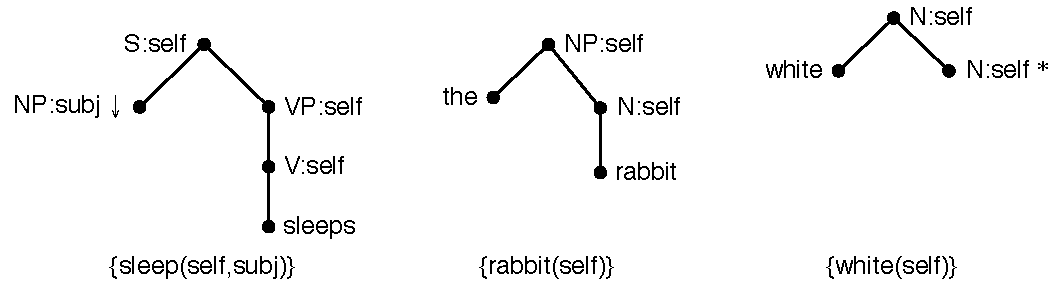
\includegraphics[width=0.75\columnwidth]{pic-grammar}
  \caption{An example grammar in the sentence generation domain.}
  \label{fig:white-rabbit-sleeps-grammar}
\end{figure}

\begin{figure}[t]
  \centering
  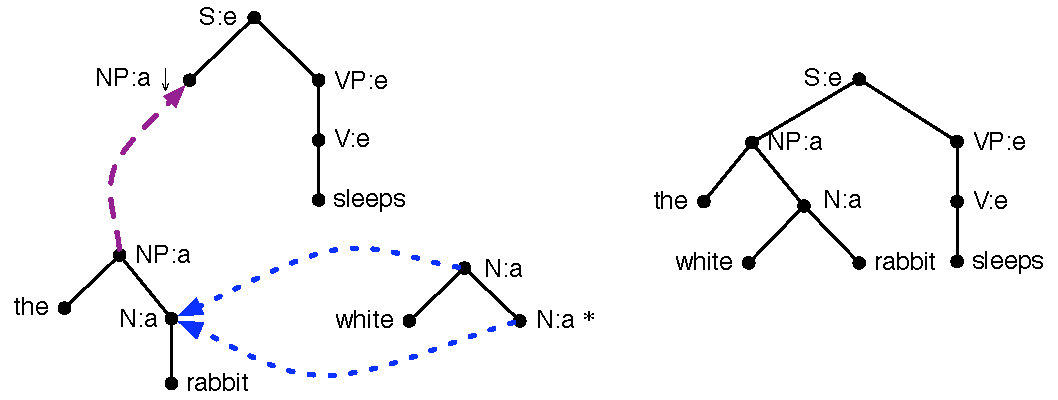
\includegraphics[width=0.75\columnwidth]{pic-derivation}
  \caption{Derivation of ``The white rabbit sleeps.''}
  \label{fig:white-rabbit-sleeps-deriv}
\end{figure}

We can now consider various different algorithms for solving the SPUD
problem. The naive algorithm builds the TAG derivation top-down. In
the example, it starts with the elementary tree for ``sleeps''. This
tree satisfies the need to convey the semantic information, but
introduces a need to generate a noun phrase (NP) for the subject,
which must refer uniquely to the target referent $r_1$. In a second
step, we substitute the tree for ``the rabbit'' into the open NP leaf,
which makes the derivation grammatically complete. Since there are two
different individuals that could be described as ``the
rabbit''---technically, $r_2$ is still a \emph{distractor} (i.e.,
based on the description ``the rabbit'', the hearer might erroneously
think that we're talking about $r_2$ and not $r_1$)---we are still not
finished. To complete the derivation, the tree for ``white'' is added
to the existing structure by an \emph{adjunction} operation, making
the derivation both syntactically and semantically complete. This
search algorithm takes worst-case exponential time because it may have
to consider many combinations of elementary trees; and in fact, the
SPUD problem generalizes the surface realization problem considered by
\citet{KolStr02} and is therefore NP-complete.


\begin{figure}[p]
\centering
\begin{minipage}{0.5\textwidth}
{\small%
\begin{verbatim}
(:action add-sleeps
   :parameters (?u - node
                ?xself - individual
                ?xsubj - individual)
   :precondition
       (and (subst S ?u)
            (referent ?u ?xself)
            (sleep ?xself ?xsubj))
   :effect 
       (and (not (subst S ?u))
            (expressed sleep ?xself ?xsubj)
            (subst NP (subj ?u))
            (referent (subj ?u) ?xsubj)
            (forall (?y - individual)
                (when (not (= ?y ?xself))
                    (distractor (subj ?u) ?y)))))

(:action add-rabbit
   :parameters (?u - node
                ?xself - individual)
   :precondition 
       (and (subst NP ?u)
            (referent ?u ?xself)
            (rabbit ?xself))
   :effect 
       (and (not (subst NP ?u))
            (canadjoin N ?u)
            (forall (?y - individual)
                (when (not (rabbit ?y))
                    (not (distractor ?u ?y))))))

(:action add-white
   :parameters (?u - node
                ?xself - individual)
   :precondition 
       (and (canadjoin N ?u)
            (referent ?u ?xself)
            (rabbit ?xself))
   :effect 
       (forall (?y - individual)
           (when (not (white ?y))
               (not (distractor ?u ?y)))))
\end{verbatim}}%
\end{minipage}
\caption{PDDL actions for generating the sentence ``The white rabbit
sleeps.''}
\label{fig:white-rabbit-as-planning}
\end{figure}

The SPUD system itself worked around this complexity by using a
greedy, incomplete search algorithm. On the other hand,
\citet{KolSto07} present an alternative to controlling the necessary
search, by encoding the generation problem into a planning
problem.\footnote{See \url{http://code.google.com/p/crisp-nlg/} for
  the CRISP system, in which this conversion is implemented.} Each
operator of this planning problem models the addition of some
elementary tree to the TAG derivation. For instance,
Figure~\ref{fig:white-rabbit-as-planning} shows the corresponding PDDL
actions for the above generation task. The \texttt{add-sleeps}
operator represents the addition of the elementary tree for ``sleeps''
to the derivation. $\verb?add-sleep?(\mathsf{root},e,r_1)$ removes the
atom $\mathsf{subst}(S,\mathsf{root})$, which expresses that there is
currently an open substitution node $\mathsf{root}$ with label $S$,
from the planning state and replaces it with an atom
$\mathsf{subst}(NP,\mathsf{subj}(\mathsf{root}))$; here
$\mathsf{subj}(\mathsf{root})$ is meant as shorthand for a fresh
individual name.\footnote{These terms, which are not valid in ordinary
  PDDL, can be eliminated by estimating an upper bound $n$ for the
  plan length, making $n$ copies of each action, ensuring that copy
  $i$ can only be applied in step $i$, and replacing the term
  $\mathsf{subj}(u)$ in an action copy by the constant
  $\mathsf{subj}_i$. Notice that $S$, $NP$, and $N$ are constants.}
At the same time, the operator records that the semantic information
$\mathsf{sleep}(e,r_1)$ has now been expressed, and introduces all
individuals except for $r_1$ as distractors for the new RE at
$\mathsf{subj}(\mathsf{root})$. These distractors can then be removed
by subsequent applications of the other two operators. By assuming an
initial state that encodes the knowledge base and contains an atom
$\mathsf{subst}(S,\emph{root})$, and a goal that contains, among
others, $\forall x \forall y. \neg \mathsf{subst}(x,y)$ and
$\mathsf{expressed}(\emph{sleep},e,r_1)$, a planner will find plans
like the following:
%
\begin{enumerate}
\item $\mathsf{add}\textsf{-}\mathsf{sleeps}(\mathsf{root}, r_1)$,
\item $\mathsf{add}\textsf{-}\mathsf{rabbit}(\mathsf{subj}(\mathsf{root}),r_1)$,
\item $\mathsf{add}\textsf{-}\mathsf{white}(\mathsf{subj}(\mathsf{root}),r_1)$.
\end{enumerate}
%
Using this plan, the grammatical derivation in
Figure~\ref{fig:white-rabbit-sleeps-deriv}, and therefore the
generated sentence ``the white rabbit sleeps'', can be systematically
reconstructed. Thus, we can solve the sentence generation problem via
the detour through planning and bring current search heuristics for
planning to bear on generation.


\subsection{Planning in instruction giving}

Let's now turn to a second recent application of planning in NLG, the
GIVE Challenge (``Generating Instructions in Virtual Environments'';
\citealt{ByrKolStrCasDalMooObe09}). The object of this shared task is
to build an NLG system which produces natural-language instructions
which will guide a human user in performing some task in a virtual
environment.  From an NLG perspective, GIVE makes for an interesting
challenge because it is a theory-neutral task that exercises all
components of an NLG system, and emphasizes the study of communication
in a (simulated) physical environment. Another advantage is that GIVE
makes it possible to connect NLG systems to users over the Internet,
and thus offer cheap access to human experimental subjects. The first
installment of GIVE (GIVE-1) evaluated five NLG systems on the
performance of 1143 users, making it the largest NLG evaluation effort
in terms of human users ever.

\begin{figure}[t]
\centering
%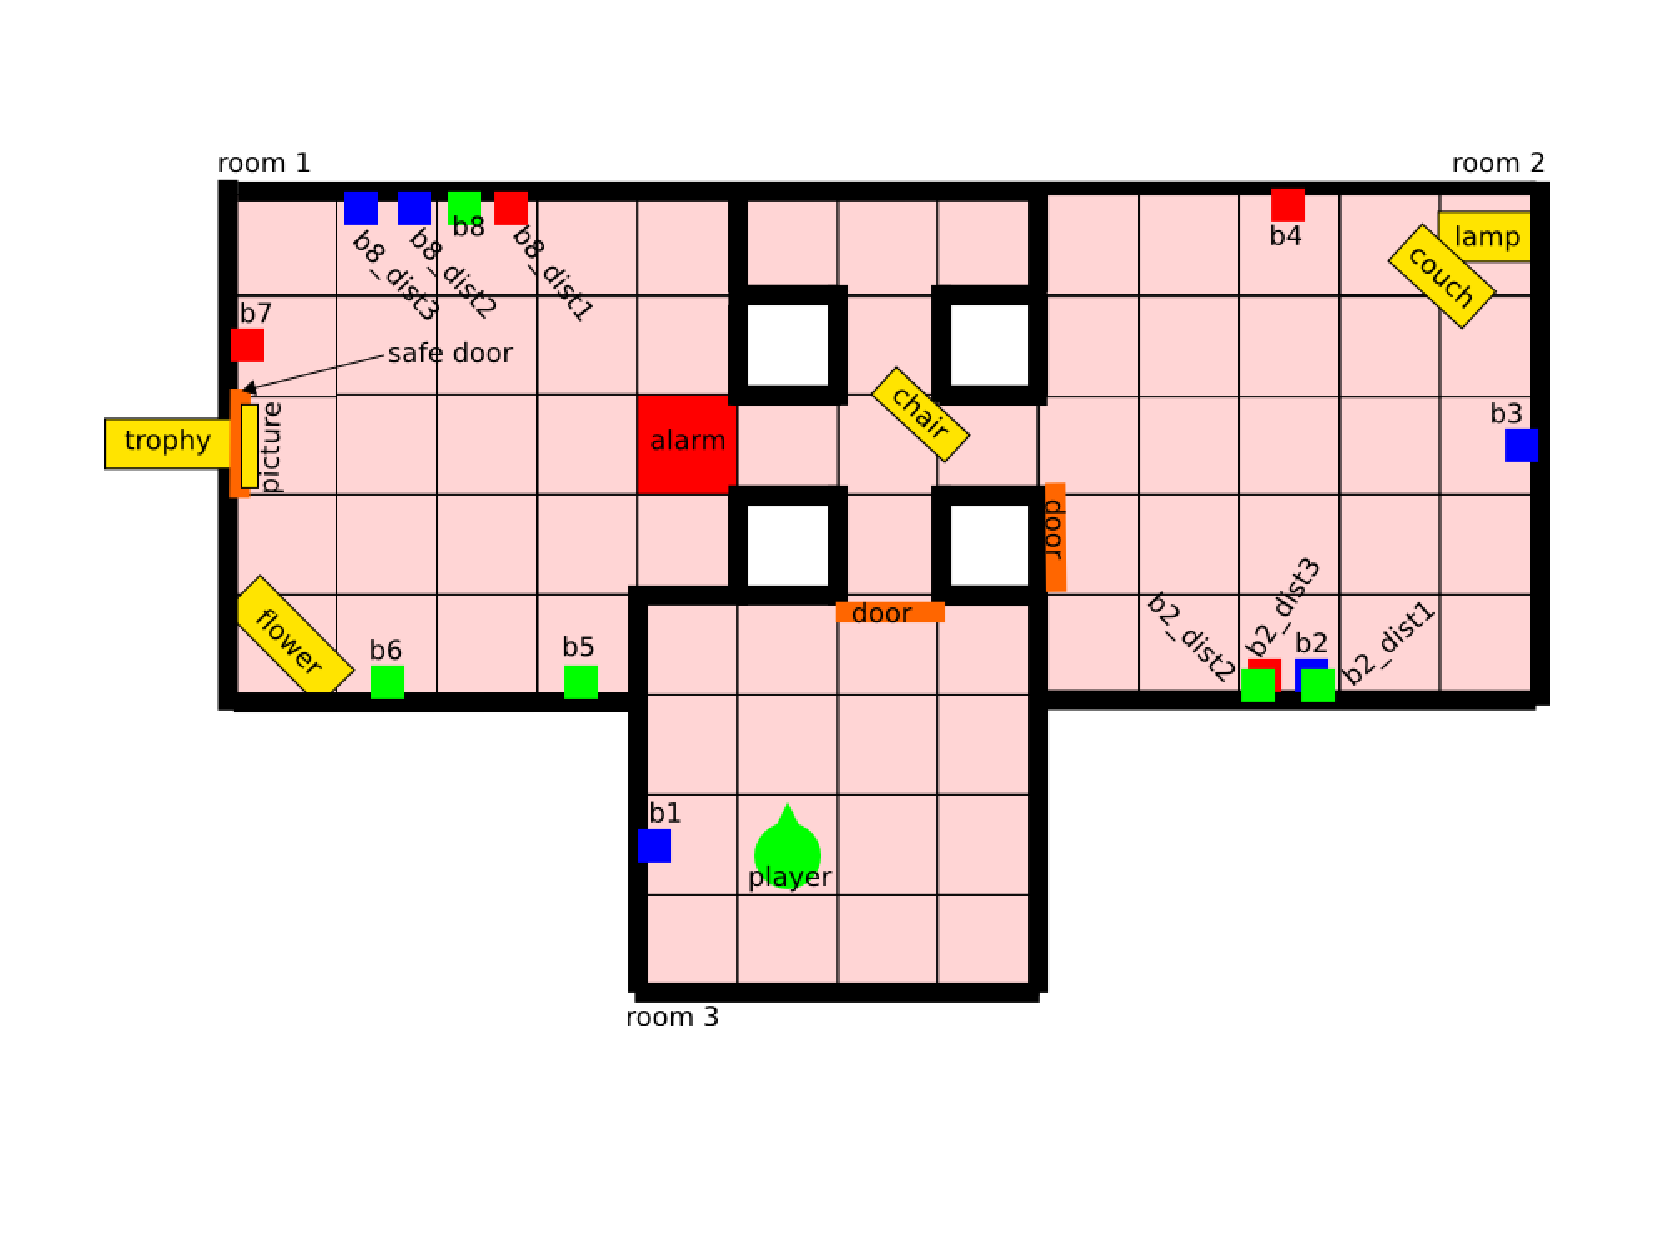
\includegraphics[width=1 \columnwidth]{give_world_no_expl}
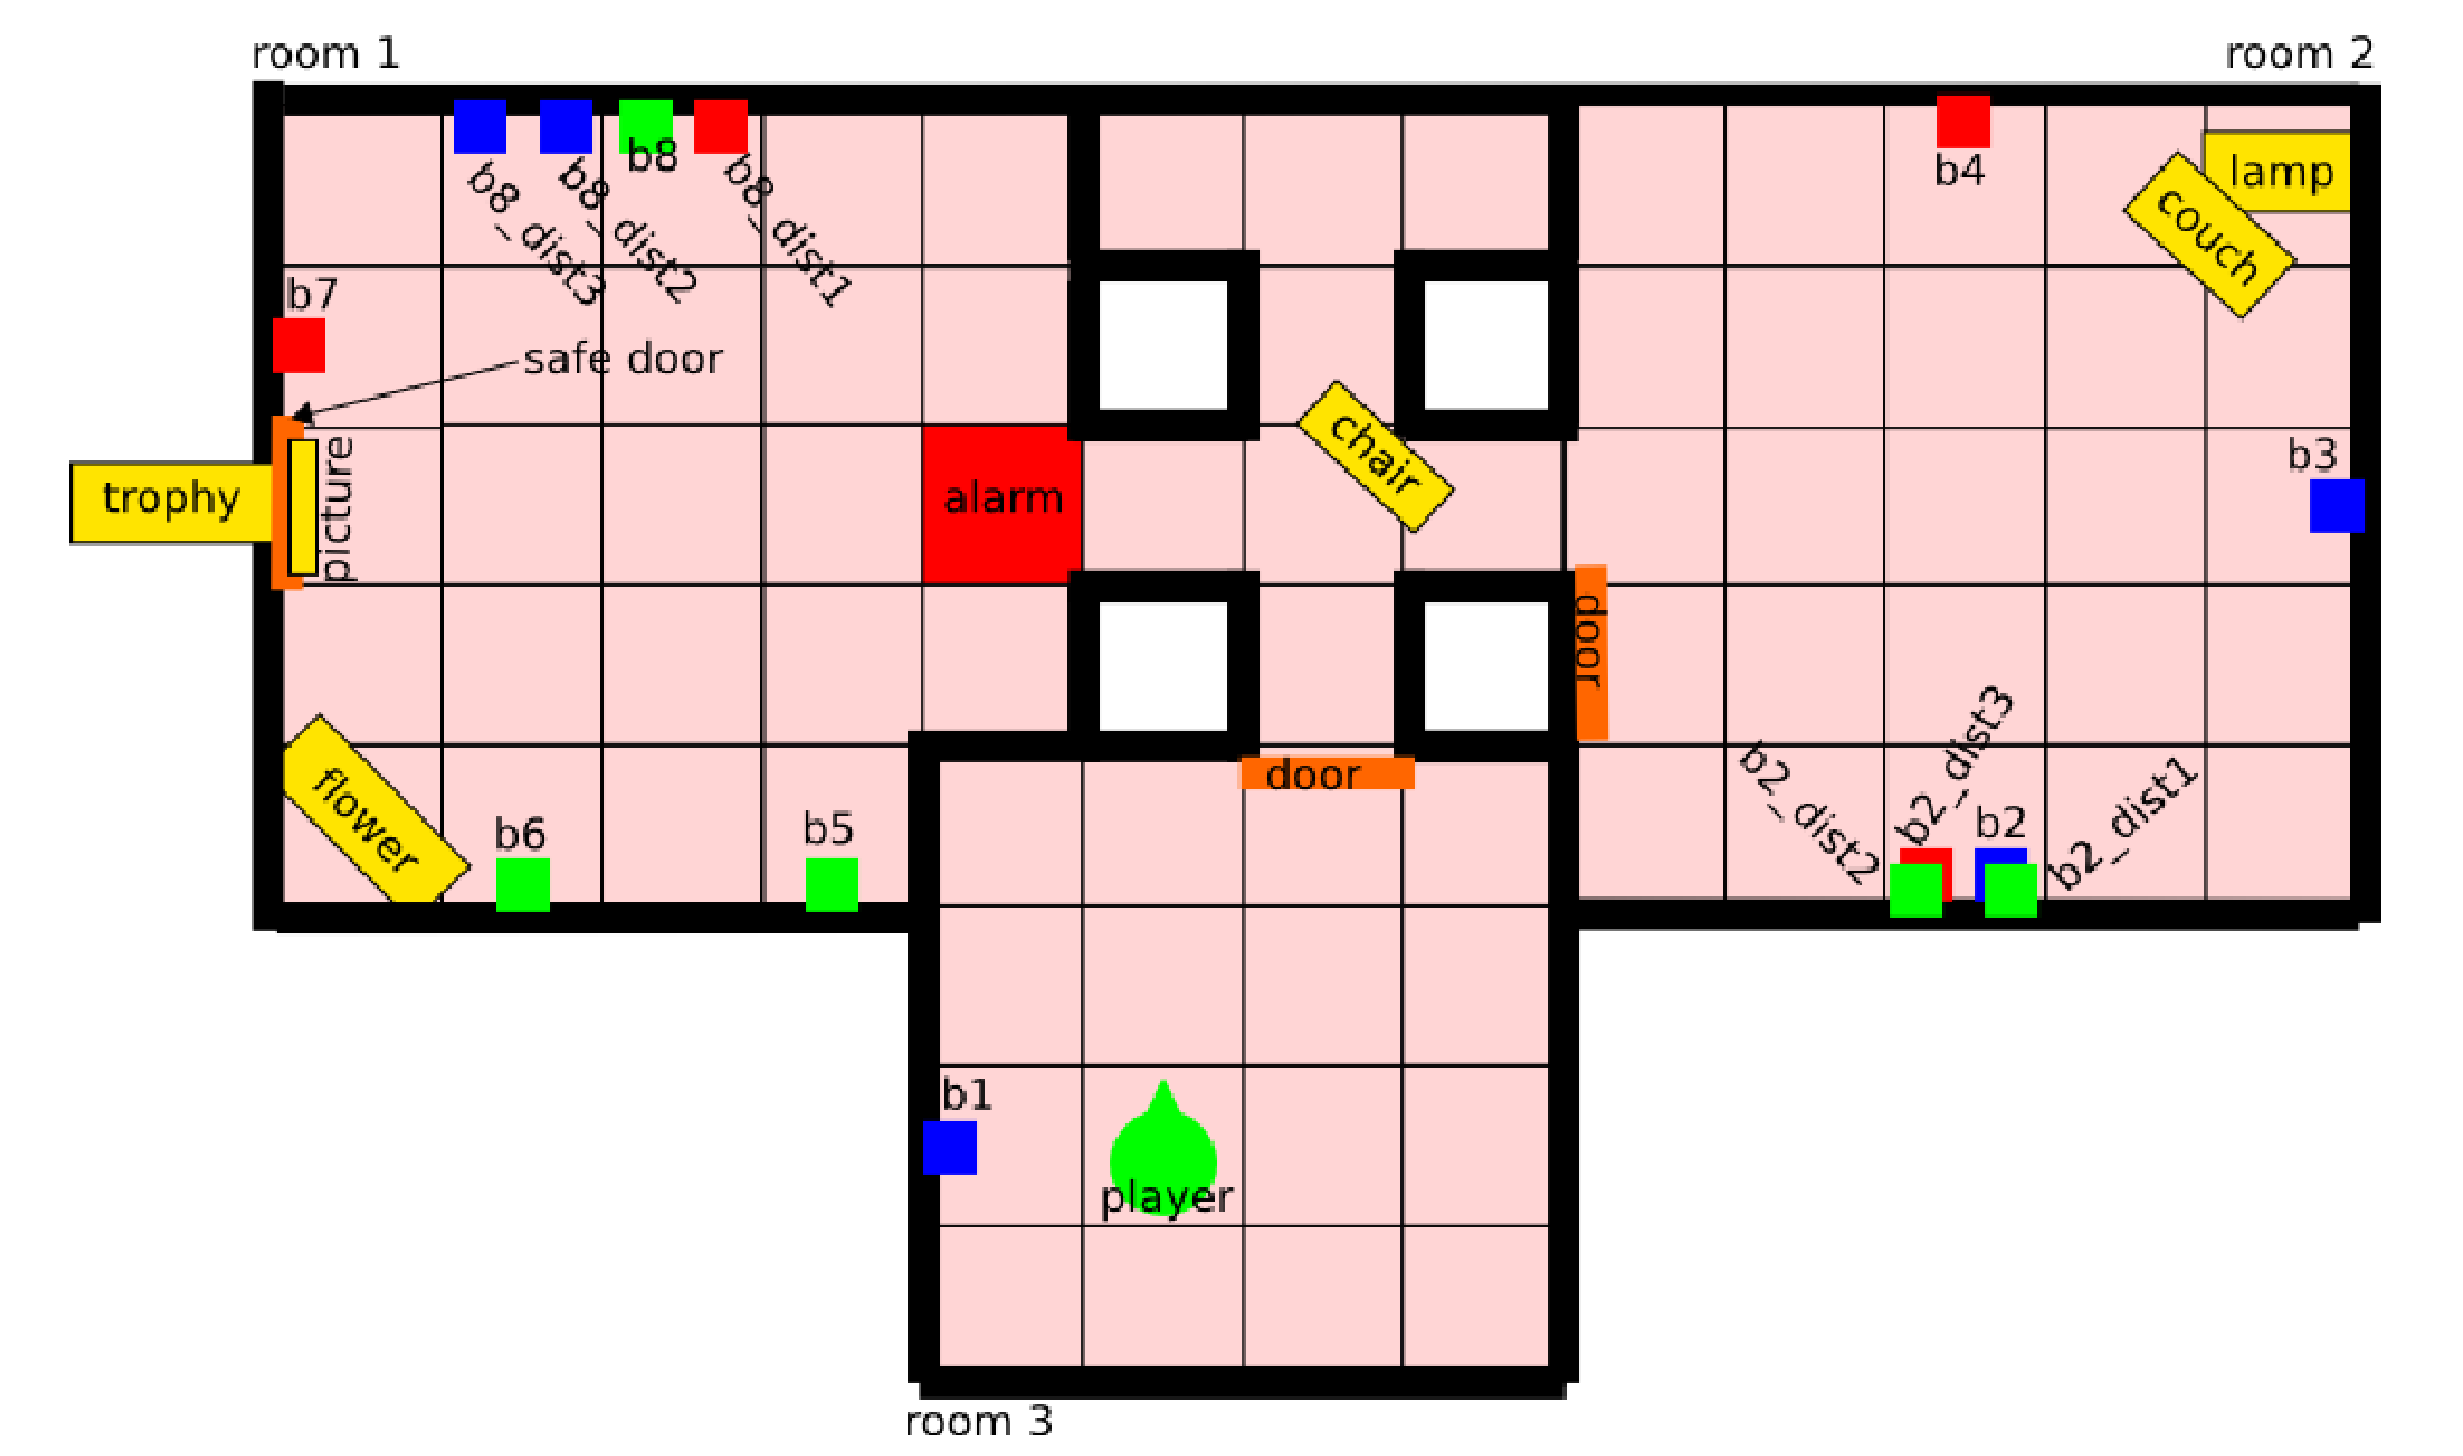
\includegraphics[width=0.75\columnwidth]{give_world_2}
\caption{Map of a GIVE world.}
  \label{fig:give-development-world}
\end{figure}

Planning plays a central role in the GIVE task. To see this, consider
the example GIVE world map in
Figure~\ref{fig:give-development-world}. To simplify both the planning
and the NLG task, this world is discretised into a set of tiles of
equal size.  The user can turn by 90 degree steps in either direction,
and can move from the centre of one tile to the centre of the next
tile, provided the path between two tiles is not blocked. The world
also consists of a set of objects which can be manipulated by the user
in various ways. For instance, in the example world the user's task is
to pick up a trophy in the top left room. The trophy is hidden in a
safe behind a picture; to access it, the user must push certain
buttons in order to move the picture out of the way, open the safe,
and open doors. Figure~\ref{fig:give-planning} shows the encoding of
some of the available GIVE domain actions, in PDDL syntax. In the
example, the shortest plan to solve the task consists of 108 action
steps, with the first few steps as follows:
%
\begin{enumerate}
\item $\mathsf{turn}\textsf{-}\mathsf{left}(\mathsf{north},
\mathsf{west})$,
\item $\mathsf{move}(\mathsf{pos\_5\_2}, \mathsf{pos\_4\_2}, \mathsf{west})$,
\item $\mathsf{manipulate}\textsf{-}\mathsf{b1}\textsf{-}\mathsf{off}\textsf{-}\mathsf{on}(\mathsf{pos\_5\_2})$,
\item $\mathsf{turn}\textsf{-}\mathsf{right}(\mathsf{west}, \mathsf{north})$.
\end{enumerate}

\begin{figure}[p]
\centering
\begin{minipage}{0.5\textwidth}
{\small%
\begin{verbatim}
(:action move
   :parameters (?from - position
                ?to - position
                ?ori - orientation)
   :precondition 
       (and (player-pos ?from) 
            (adjacent ?from ?to ?ori) 
            (player-orient ?ori)
            (not-blocked ?from ?to)
            (not-alarmed ?to))
   :effect 
       (and (not (player-pos ?from))
            (player-pos ?to)))

(:action turn-left
   :parameters (?ori - orientation
                ?newOri - orientation)
   :precondition 
       (and (player-orient ?ori)
            (next-orient-left ?ori ?newOri))
   :effect 
       (and (not (player-orient ?ori))
            (player-orient ?newOri)))

(:action turn-right
   :parameters (?ori - orientation
                ?newOri - orientation)
   :precondition 
       (and (player-orient ?ori)
            (next-orient-right ?ori ?newOri))
   :effect 
       (and (not (player-orient ?ori))
            (player-orient ?newOri)))

(:action manipulate-b1-off-on
   :parameters (?pos - position)
   :precondition 
       (and (state b1 off)
            (player-pos ?pos)
            (position b1 ?pos))
   :effect 
       (and (not (state b1 off))
            (state b1 on)
            (not (state d1 closed))
            (state d1 open) 
            (not (blocked pos_6_5 pos_6_4))
            (not (blocked pos_6_4 pos_6_5))))
\end{verbatim}}%
\end{minipage}
\caption{Some PDDL actions for the GIVE domain.}
\label{fig:give-planning}
\end{figure}

A GIVE NLG system must be able to compute such plans. At a minimum,
the discourse planner will call a planner in order to determine the
content of the instructions that should be presented to the
user. Under this view, the planning problem is very similar to the
Gridworld problem (see, e.g., \citep{Tovey-Koenig:2000}), which also
involves finding a route through a two-dimensional world map with
discrete positions. GIVE tasks are usually much more complex, however,
as illustrated by the above example map: a successful plan must
include steps for pressing buttons in the right order, reasoning about
large numbers of world objects, and navigating through complicated
room shapes. This relatively loose integration of NLG system and
planner is the state of the art of the systems that participated in
GIVE-1.

However, in order to solve the GIVE task in a more satisfying way, we
expect that planning and generation will have to be interleaved more
closely, making the planning a genuine part of the NLG task. For
instance, the NLG system could generate an instruction sequence
starting with ``turn left; walk forward; press the button; turn right;
walk forward; walk forward; turn right; walk forward; walk forward;
turn left; walk forward''. But such instructions are clumsy and
uninteresting; it would be much better to say ``turn around and walk
through the door''. That is, the system should \emph{summarise} plans
by merging multiple action instances into single instructions before
presenting them to the user.\footnote{This task is similar to the
  construction of ``macro'' actions, but is primarily intended for
  plan presentation purposes. See, e.g., \citep{Botea-etal:05} which
  contains a survey of recent approaches for generating macro actions
  in planning.}  Conversely, it may also be necessary to
\emph{elaborate} on a single planning step by expressing it with
several instructions. Having just entered the top left room, it may be
easier for the user to understand the instruction ``walk to the centre
of the room; turn right; now press the green button in front of you'',
rather than the instruction ``press the green button on the wall to
your right''. Furthermore, in order to plan the referring expression
``the green button in front of you'' at a time when the button is not
yet in front of the user, the NLG system must keep track of the
hypothetical changes in what objects are visible to the user. Thus,
the NLG acts of referring and instructing must be tightly integrated
with the modules for plan generation. This makes the GIVE domain
planning problem an integral part of the NLG system, which makes this
a second planning problem of immediate relevance to NLG that is
completely different from the first one.

% It seems to me that this paragraph misses the point. We're not
% trying to sell GIVE as a cool problem here; we take the perspective
% that GIVE exists and has already been shown to be cool, and we only
% talk about solving it here. - AK
%
% From a planning perspective, GIVE imposes very strict runtime
% requirements on the plan generation task: planning must
% happen in real time and the system must respond to a user in a timely
% fashion.  If the system takes too much time deliberating over an
% instruction to give, rather than actually giving this instruction, the
% user may have walked or turned away, thus making the instruction
% invalid.  Furthermore, plan execution monitoring also plays an
% important role in the GIVE problem.  At a high level, the system needs
% to monitor a user's actions and compare them against the generated
% instruction set to determine if the user has correctly followed
% directions or not. In the case of the latter, new instructions may
% have to be generated. In practice, the situation can be quite
% complicated since the mental state of the user is not known and so the
% system must be inferred from observing the user's actions in real
% time. For example, a user directed to ``turn around and walk through
% the door'' may not necessarily perform these actions to the letter,
% i.e., immediately turning 180 degrees and proceeding directly to the
% door. Instead, the user might take a roundabout route through the
% room, eventually exiting out the door.  Although the user's actions do
% not match the generated instructions exactly, they meet the intended
% goal. The system must be able to identify such ``equivalent'' plans
% and not immediately generate new instructions as soon as the user's
% actions have gone off course. Furthermore, a user can communicate
% certain intentions to the system, both through action and
% inaction. For instance, the system should infer that a user has failed
% to follow instructions if the user exits a room when given a directive
% to ``walk to the centre of the room''. The system should also make a
% similar conclusion if a user simply does nothing when given the
% instruction.


\section{Experiments}
\label{sec:experiments}

We now describe the results of four simple experiments designed to evaluate
the performance of three planners---FF \citep{HoffmannNebel01}, SGPLAN
5.2.2 \citep{hsu06:_new_featur_in_sgplan_for}, and an ad-hoc implementation
of GraphPlan \citep{Blum1997} written in Java---in our NLG domains. The FF
and SGPLAN planners were chosen due to their success in the International
Planning Competitions. Our implementation of GraphPlan is included as a
counterpoint to the other two, more complex, planners. Most notably, our
version of GraphPlan does not perform a preprocessing ``grounding'' step
like FF and SGPLAN but is much more selective in its predicate and action
instantiations.

On first impressions, our results indicate that planning is a promising
tool for both domains.  In the sentence generation domain, FF dramatically
outperforms the best previously known algorithm for the same problem (a
reimplementation of \citep{Stone2003a}), although the latter approach uses
a greedy search algorithm with a heuristic that is hand-tailored to the
domain. In the GIVE domain, SGPLAN computes a domain plan from the initial
state to the goal in 0.3 seconds, which is fast enough for moderately-sized
problems instances in the application.\footnote{All
  runtimes were measured on a Pentium 4 CPU running at 3 GHz. Java programs
  were allowed to ``warm up'', i.e., the planner was run five times and the
  first four measurements discarded to ensure that the JVM had just-in-time
  compiled all relevant bytecode.}

We also observe that although FF and SGPLAN manage the search for plans
very efficiently, they both spend comparatively large amounts of time
computing predicate and action instantiations in their preprocessing
stages, many of which are then never used during the search. FF's
``grounding time'' in particular dominates its overall planning time,
leading to some conflicting results. In some cases, our Java implementation
of GraphPlan significantly outperforms both state-of-the-art planners. The
experiments described below seek to improve our understanding of this
situation.


\subsection{Experiment 1: Sentence generation}
\label{sec:exper-1:-sent}

In the first experiment, we construct a series of sentence generation
problems which require the planner to compute a plan representing the
sentence ``Mary likes the Adj$_1$ \ldots Adj$_n$ rabbit.''  Each problem
instance assumes a certain number $m$ of rabbits that were distinguished by
$n \leq m$ different properties, such that all $n$ properties are required
to distinguish the target referent from all other rabbits.  The $n$
properties are realized as $n$ different adjectives, in any order.  This
setup allows us to control the plan length (a plan with $n$ properties will
have length $n+4$) and the universe size (the universe will contain $m+1$
individuals in addition to the differently-typed individuals used to encode
the grammar).

\begin{figure}
  \centering
  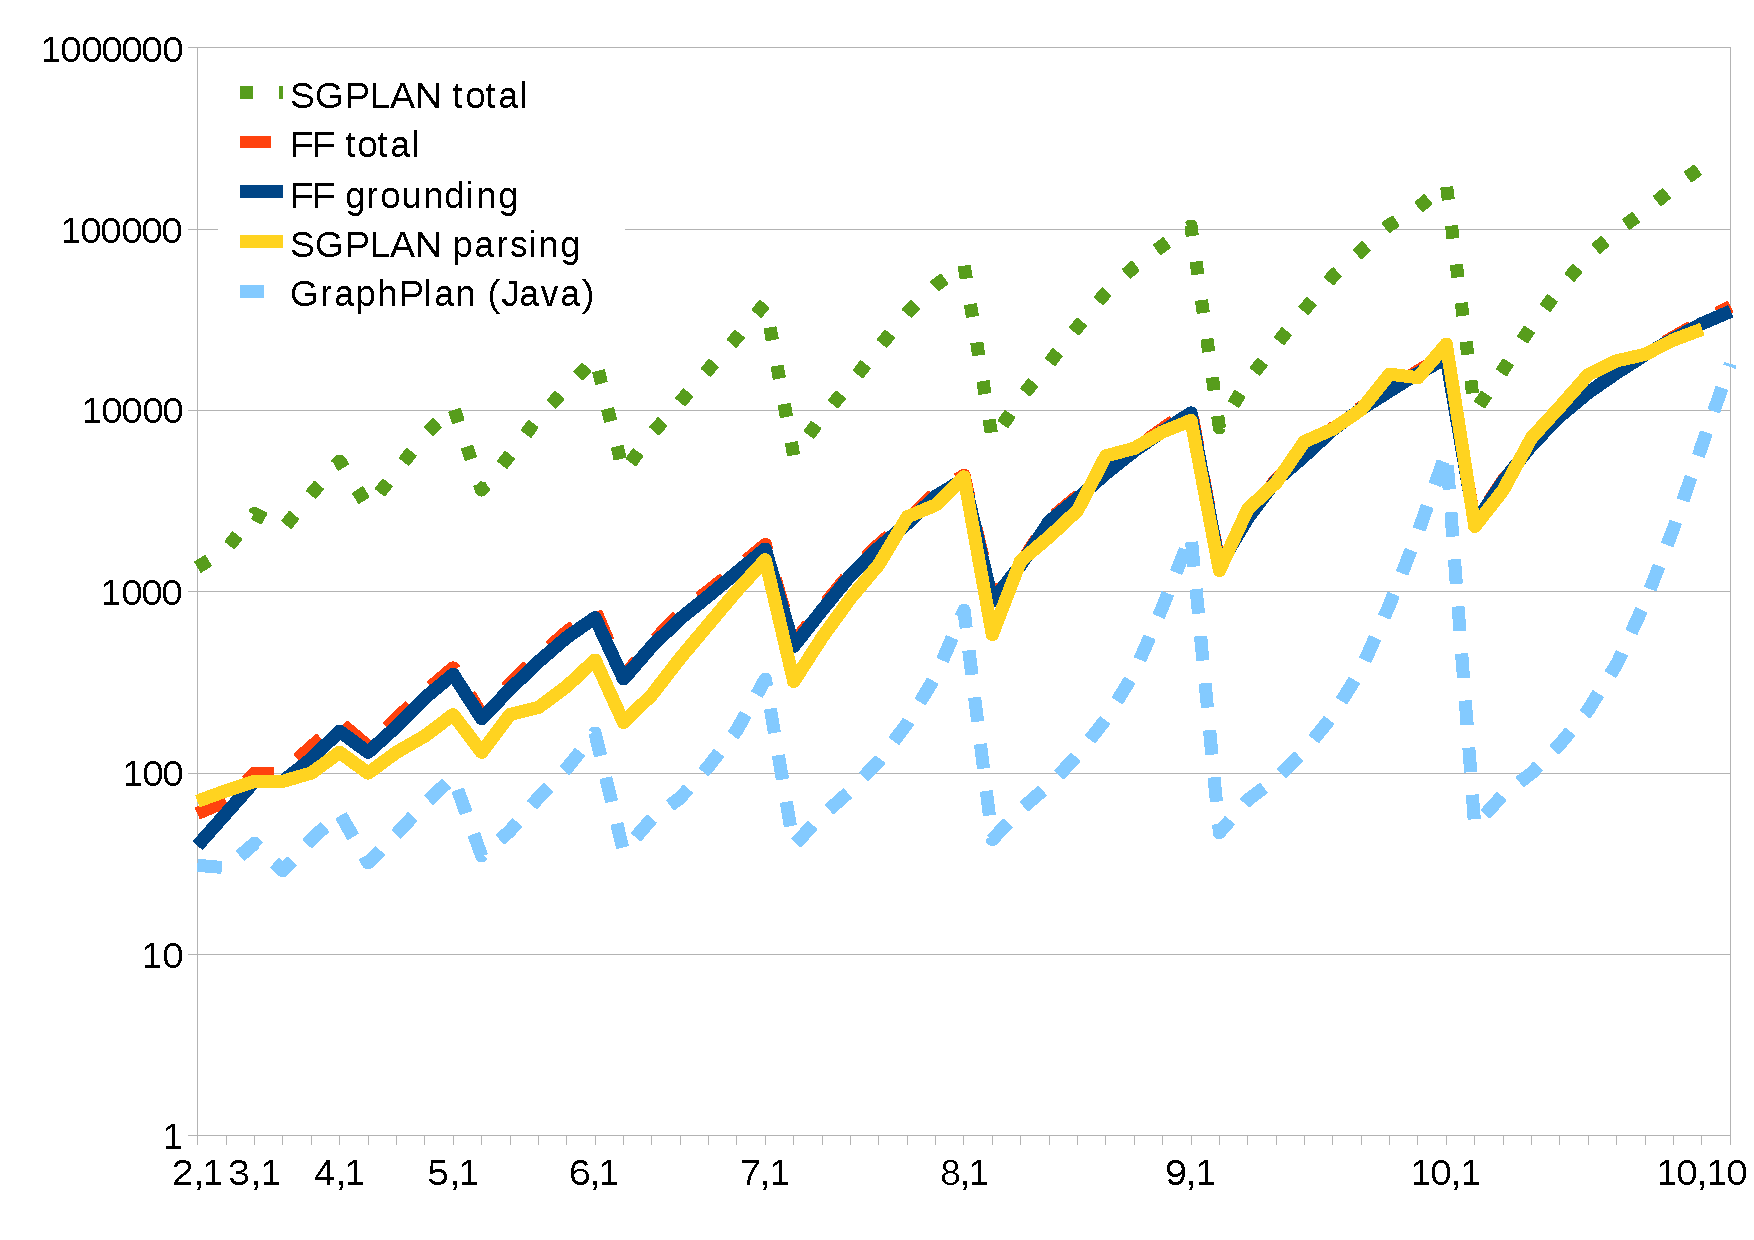
\includegraphics[width=0.75\columnwidth]{graph-exp1}
  %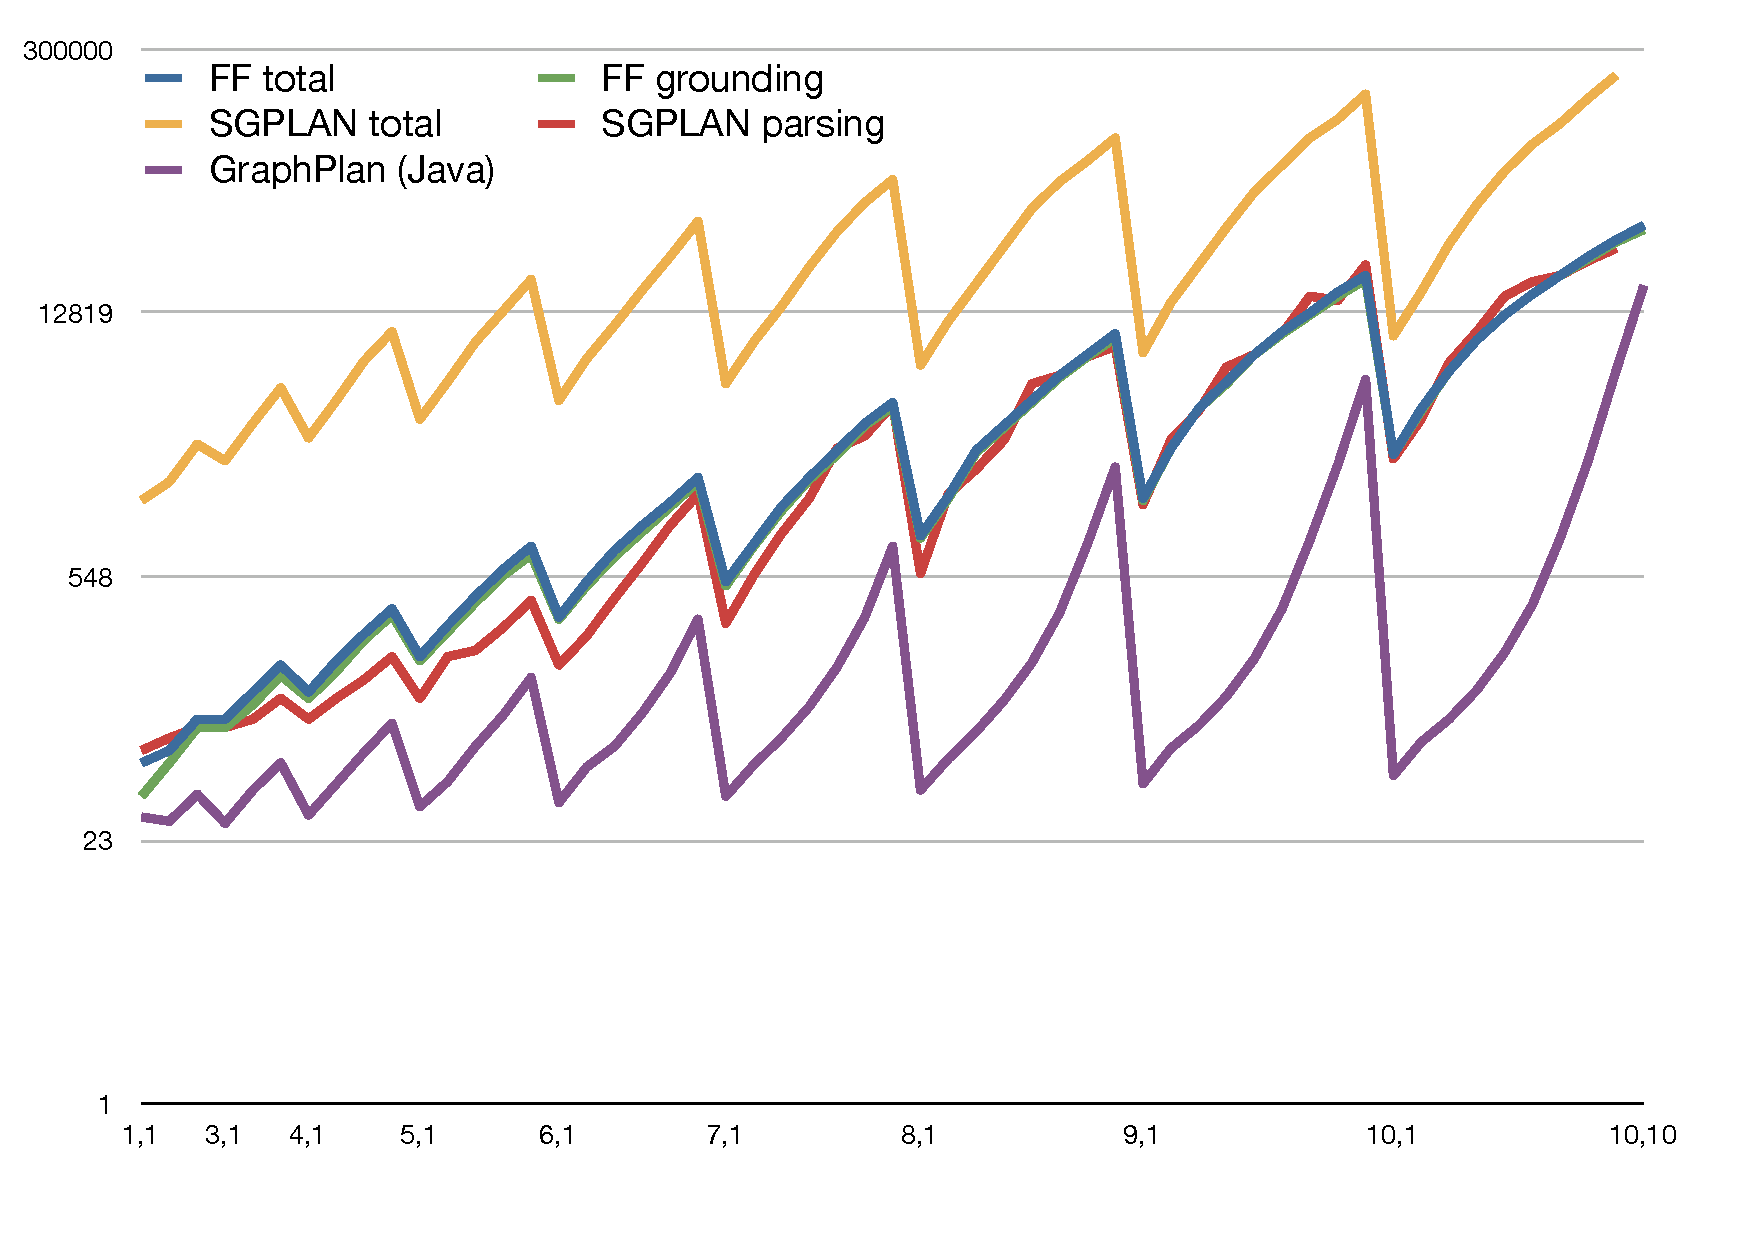
\includegraphics[width=1\columnwidth]{pic-runtime-modifiers-with-sgplan}
  \caption{Results for the sentence generation domain. The
    horizontal axis represents parameters $(m,n)$ from $(1,1)$ to
    $(10,10)$ in lexicographical order. The vertical axis is the
    runtime in milliseconds.}
  \label{fig:runtimes-crisp}
\end{figure}

The results of this experiment are shown in the graph in
Figure~\ref{fig:runtimes-crisp}. The input parameters $(m,n)$ are plotted
in lexicographic order on the horizontal axis and the runtime is shown in
milliseconds on the vertical axis. These results reveal a number of
interesting insights. First, FF significantly outperforms SGPLAN in this
domain, sometimes by a factor of 10 or more.\footnote{Experiments with
 SGPLAN use a pre-release version of SGPLAN, kindly provided to us by
 Chih-Wei Hsu.The release version of SGPLAN 5.2.2 had a bug which caused it
 to crash on some of our problem instances.}
Second, FF's runtime is dominated by its initial grounding step, in which
it computes the ground instances of all predicates and actions used in the
planning problem in order to avoid unnecessary instantiation during search.
In particular, the ratio of grounding time to total runtime is generally
above 85\%, and rises to above 99\% at $m=11$, which is still a relatively
small universe for this application.\footnote{The
  ``grounding'' time reported here is what FF reports as ``time spent:
  instantiating action templates''.} 

In our testing examples, the time spent by FF on grounding is such that it
is consistently outperformed by our Java implementation of GraphPlan, which
only computes instances of predicates and actions as they are discovered
during the construction of the planning graph. Although FF is consistently
much faster as far as pure search time is concerned, our results indicate
that FF's performance is much more sensitive to the domain size: if we fix
$n=1$, FF takes 60 ms to compute a plan at $m=1$, but 2.4 seconds to
compute the same plan at $m=10$. By comparison, our GraphPlan
implementation takes 30 ms at $m=1$ and still only requires 50 ms at
$m=10$. Conversely, GraphPlan's runtime grows much faster with the plan
size (i.e., with growing values of $n$ for a fixed $m$). Larger, but still
realistically-sized, instances of the sentence generation problem are still
problematic for all the planners we tested.


\subsection{Experiment 2: Minimal GIVE worlds}
\label{sec:exper-2:-minim}

In the second experiment, we evaluate the performance of the planners on
problems arising in the GIVE domain. We construct a series of test worlds,
similar to the one illustrated in Figure~\ref{fig:give-minimal}. These
worlds consist of a $2n$ by $h$ grid of positions, such that there are
buttons at positions $(2i-1,1)$ and $(2i,h)$ for $1 \leq i \leq n$. The
player starts in position $(1,1)$ and must press all the buttons
to successfully complete the game. The world is generated as a GIVE world
description, and then automatically converted into a planning problem by
the GIVE software. For instance, Figure~\ref{fig:give-planning} shows some
of the actions available in the GIVE domain in PDDL syntax.

\begin{figure}[t]
  \centering
  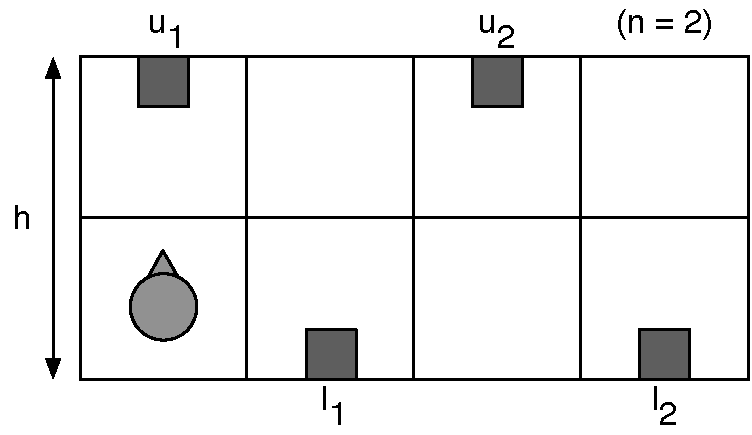
\includegraphics[width=0.5\columnwidth]{pic-buttons}
  \caption{Minimal GIVE world.}
  \label{fig:give-minimal}
\end{figure}

Results for the $h=20$ case, with $n$ ranging from $1$ to $40$, are shown
in Figure~\ref{fig:give-runtime-minimal}. The most obvious result is that
FF is unable to solve any problems beyond $n=13$ on our experimentation
machine within the memory limit of 1 GB. SGPLAN, on the other hand, solves
instances beyond $n=40$ without major problems. In this case, our
implementation of GraphPlan is unable to find any of these plans. The time
spent on grounding is not a major factor in either planner, probably
because the planners need more time to actually compute the plan---for
instance, the optimal plan for the problem $n=40$ has a length of about
1600 steps. As a concrete example, the following is a minimal plan for the
case of a $2$ by $2$ grid with $2$ buttons for the player to press (i.e.,
$n=1$, $h=2$):

\begin{enumerate}
\item $\mathsf{move}(\mathsf{pos\_1\_1},\mathsf{pos\_1\_2}, \mathsf{north})$,
\item $\mathsf{manipulate}\textsf{-}\mathsf{u1}\textsf{-}\mathsf{off}\textsf{-}\mathsf{on}(\mathsf{pos\_1\_2})$,
\item $\mathsf{turn}\textsf{-}\mathsf{right}(\mathsf{north}, \mathsf{east})$,
\item $\mathsf{move}(\mathsf{pos\_1\_2}, \mathsf{pos\_2\_2},
  \mathsf{east})$,
\item $\mathsf{turn}\textsf{-}\mathsf{right}(\mathsf{east}, \mathsf{south})$,
\item $\mathsf{move}(\mathsf{pos\_2\_2}, \mathsf{pos\_2\_1}, \mathsf{south})$,
\item $\mathsf{manipulate}\textsf{-}\mathsf{l1}\textsf{-}\mathsf{off}\textsf{-}\mathsf{on}(\mathsf{pos\_2\_1})$.
\end{enumerate}


\begin{figure}[t]
  \centering
  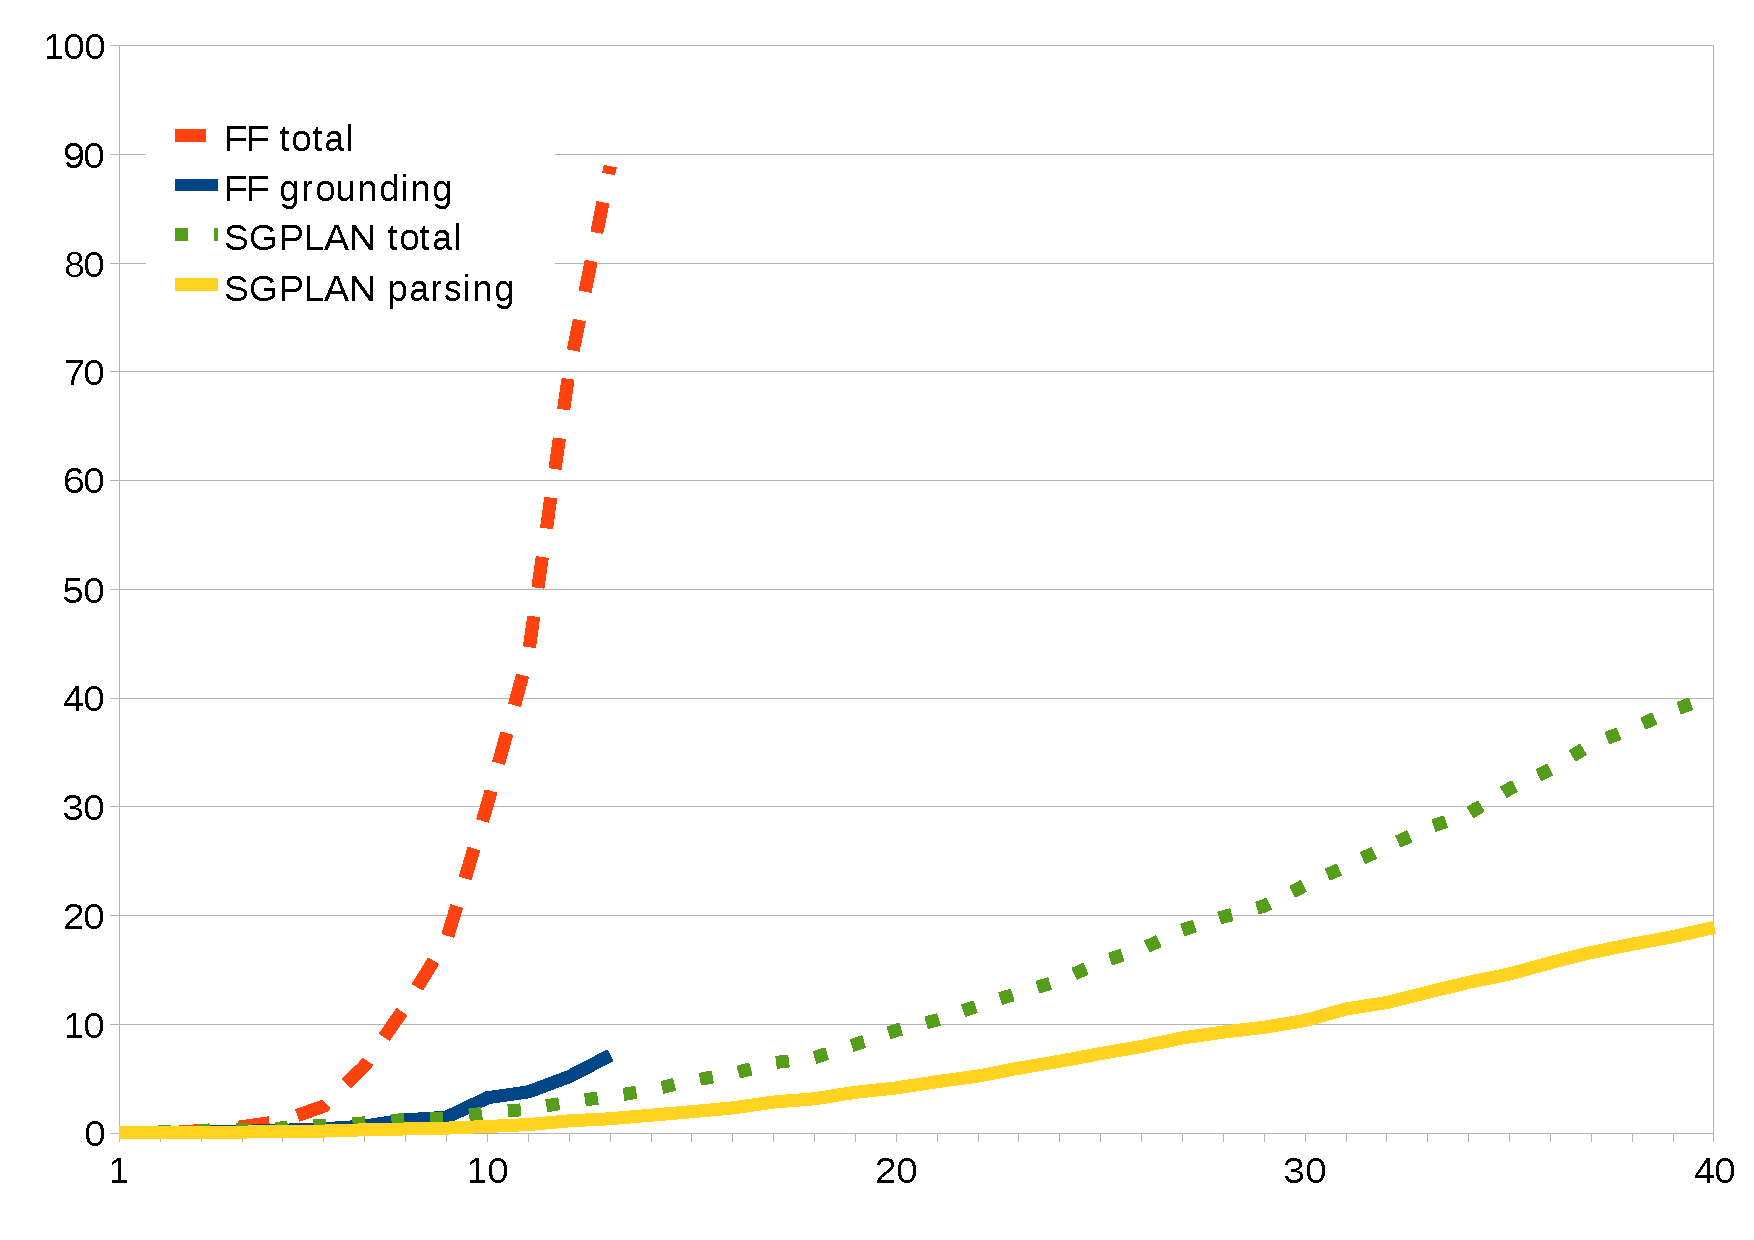
\includegraphics[width=0.75\columnwidth]{graph-exp2}
  %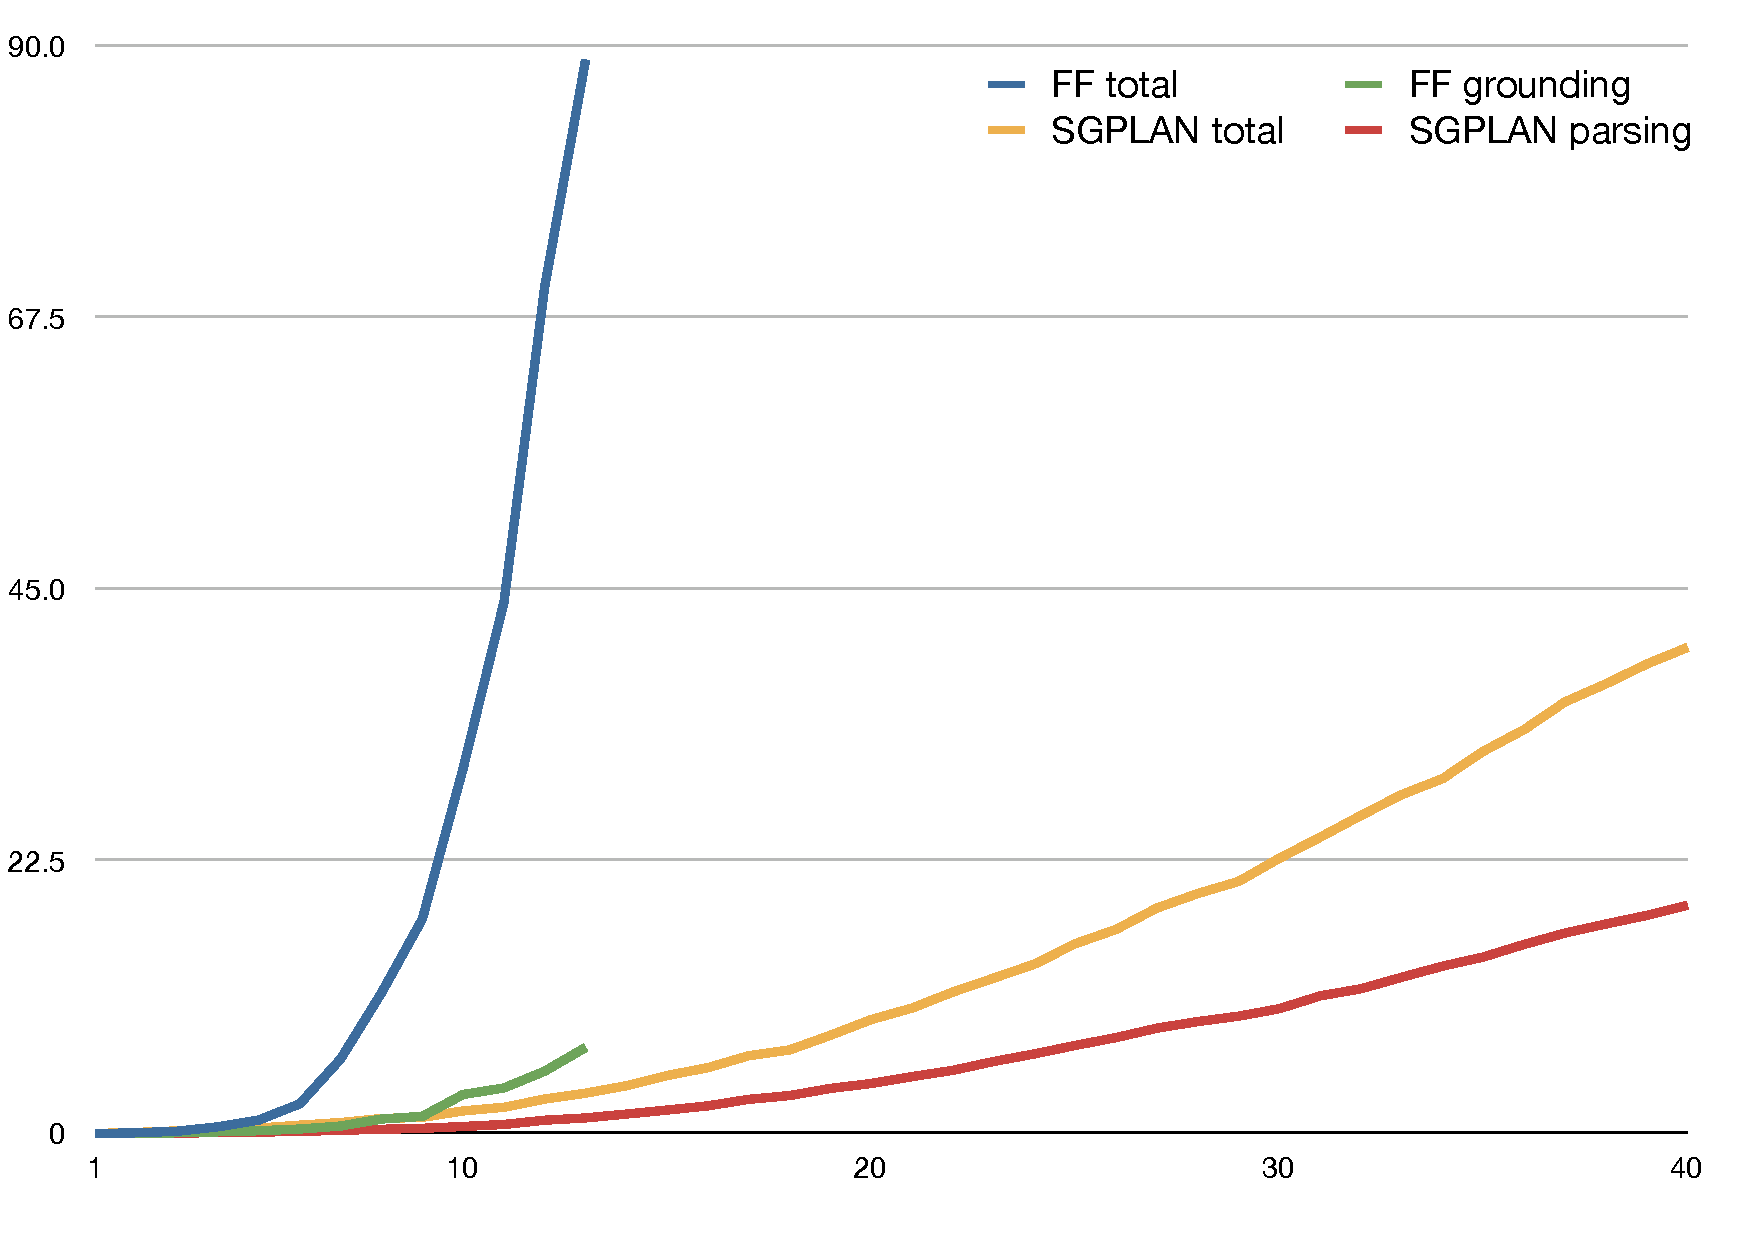
\includegraphics[width=1\columnwidth]{pic-runtime-buttons}
  \caption{Results on the minimal GIVE
    domain for $h=20$. The horizontal axis is $n$. The vertical axis
    is the runtime in seconds.}
  \label{fig:give-runtime-minimal}
\end{figure}


\subsection{Experiment 3: GIVE worlds with extra positions}
\label{sec:experiment-3:-give}

In the third experiment, we vary the structure of the GIVE world in order
to judge the effect that universe size has on the planning problem in this
domain. Starting with the ordinary GIVE world described in Experiment~2, we
extend the world map by adding another $w$ by $h$ empty ``junk'' positions
to the right of the minimal world, as shown in Figure~\ref{fig:give-junk}.
These new positions are not actually required in any plan, but extend the
size of the state space and approximate the situation in the actual GIVE
domain where most grid positions are never used. We leave the initial state
and goal untouched. As before, we generate a GIVE world description and
then convert it into a planning problem in PDDL.

\begin{figure}[t]
  \centering
  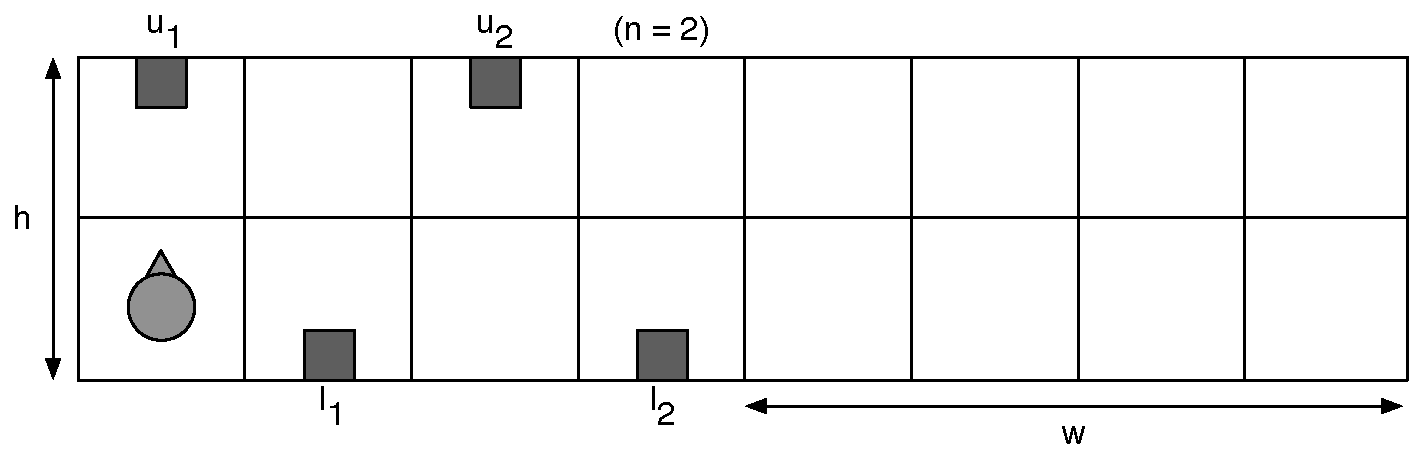
\includegraphics[width=0.80\columnwidth]{pic-empty-buttons}
  \caption{GIVE world with extra ``junk'' positions.}
  \label{fig:give-junk}
\end{figure}

Results for the $h=20$, $n=5$ case with $w$ ranging from $1$ to $70$ are
shown in Figure~\ref{fig:give-runtime-junk}. As in Experiment~2, FF again
runs out of memory, this time at $w=17$, while SGPLAN easily solves inputs
beyond $w=70$. As in Experiment~2, our implementation of GraphPlan is
unable to generate any of these plans. Unlike Experiment 2, however, both
FF and SGPLAN now spend a substantial proportion of their time on
grounding. In SGPLAN, this translates to a ``parsing time'' (which we
assume includes grounding) which grows from 180 ms to 21.7 seconds as $w$
grows from $1$ to $75$. The rest of the runtime, which also includes the
search time, only grows from 400 ms to 2.3 seconds. This difference is
particularly dramatic given that the actual optimal plan in each case is an
identical plan of about 100 steps (i.e., the one we would have found in
Experiment 2 for the $h=20$, $n=5$ case). The planning times for these
instances are also concerning since times over a couple seconds will
negatively affect the overall response time of the system, which must react
in real time to user actions.

\begin{figure}[t]
  \centering
  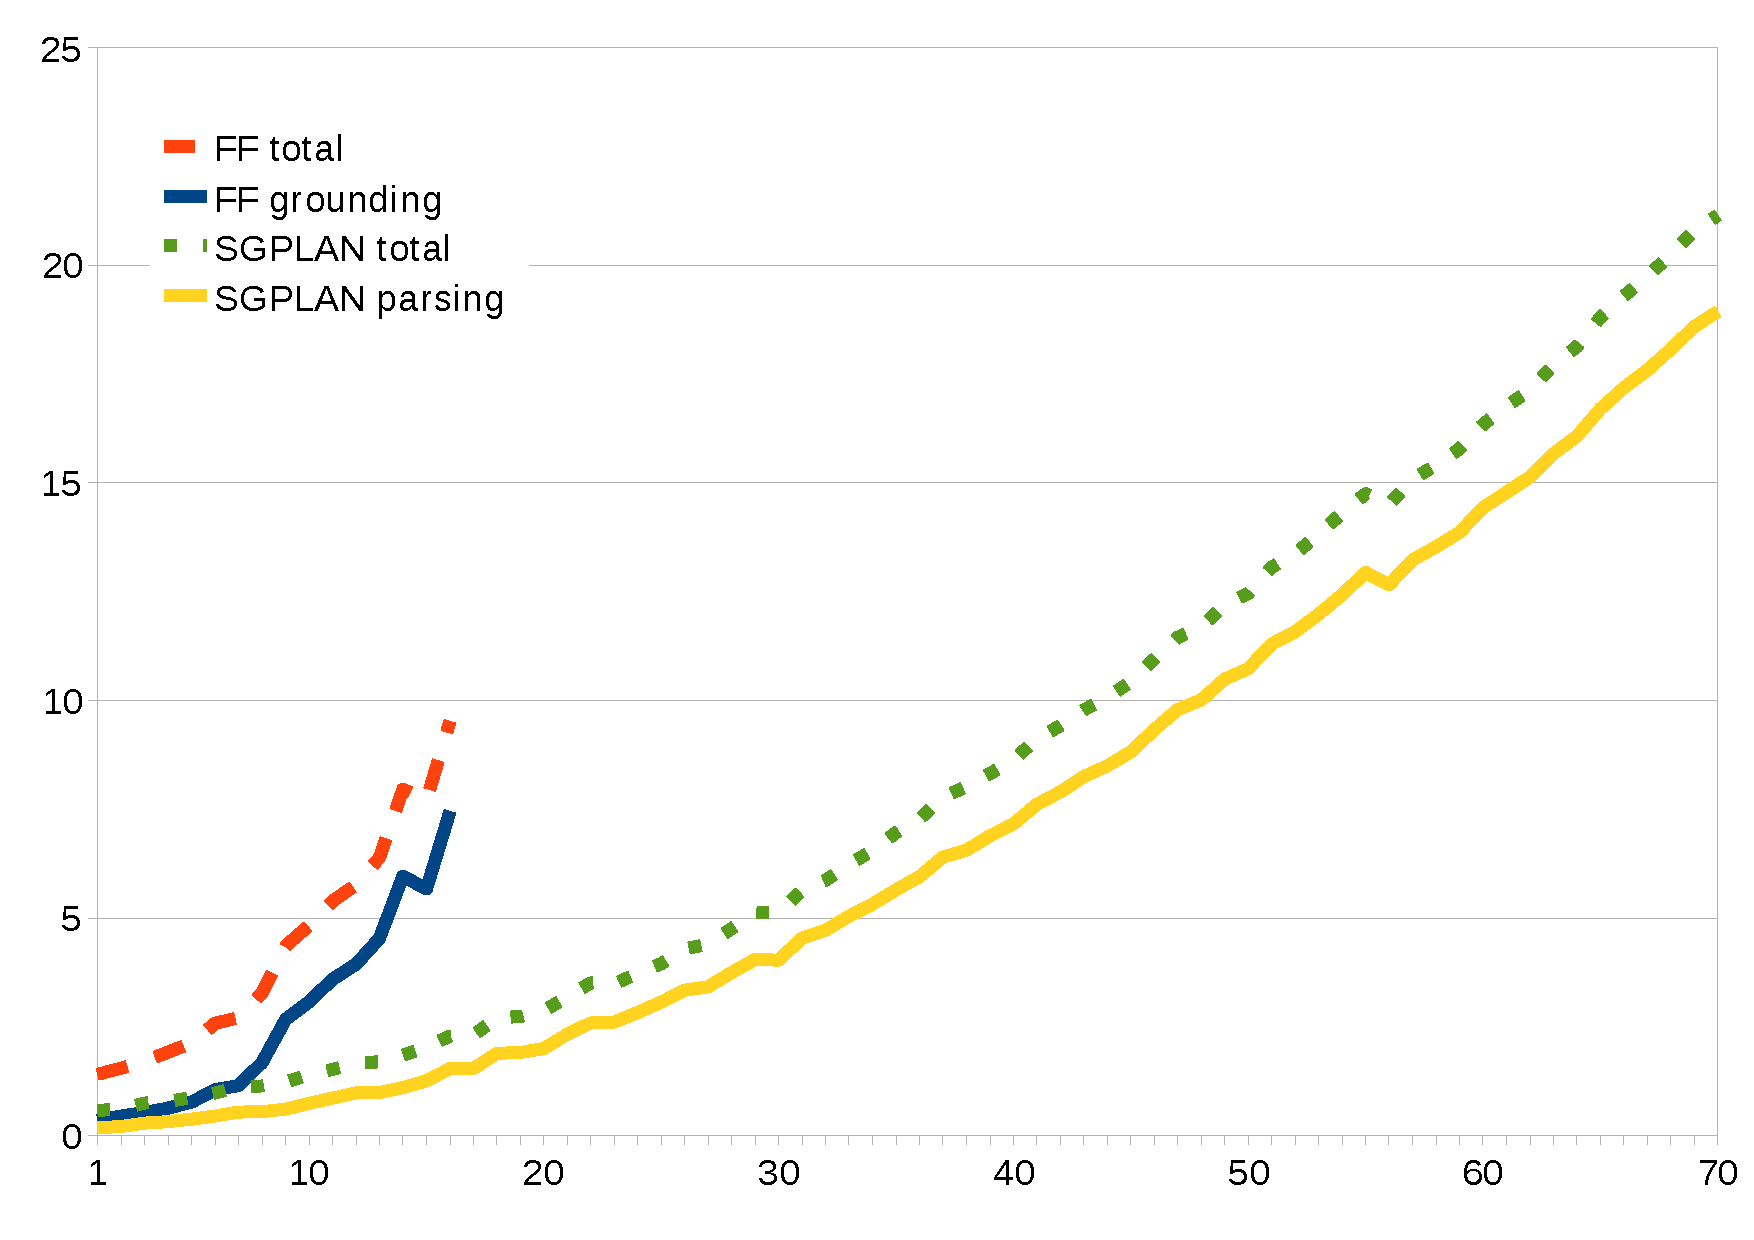
\includegraphics[width=0.75\columnwidth]{graph-exp3}
  %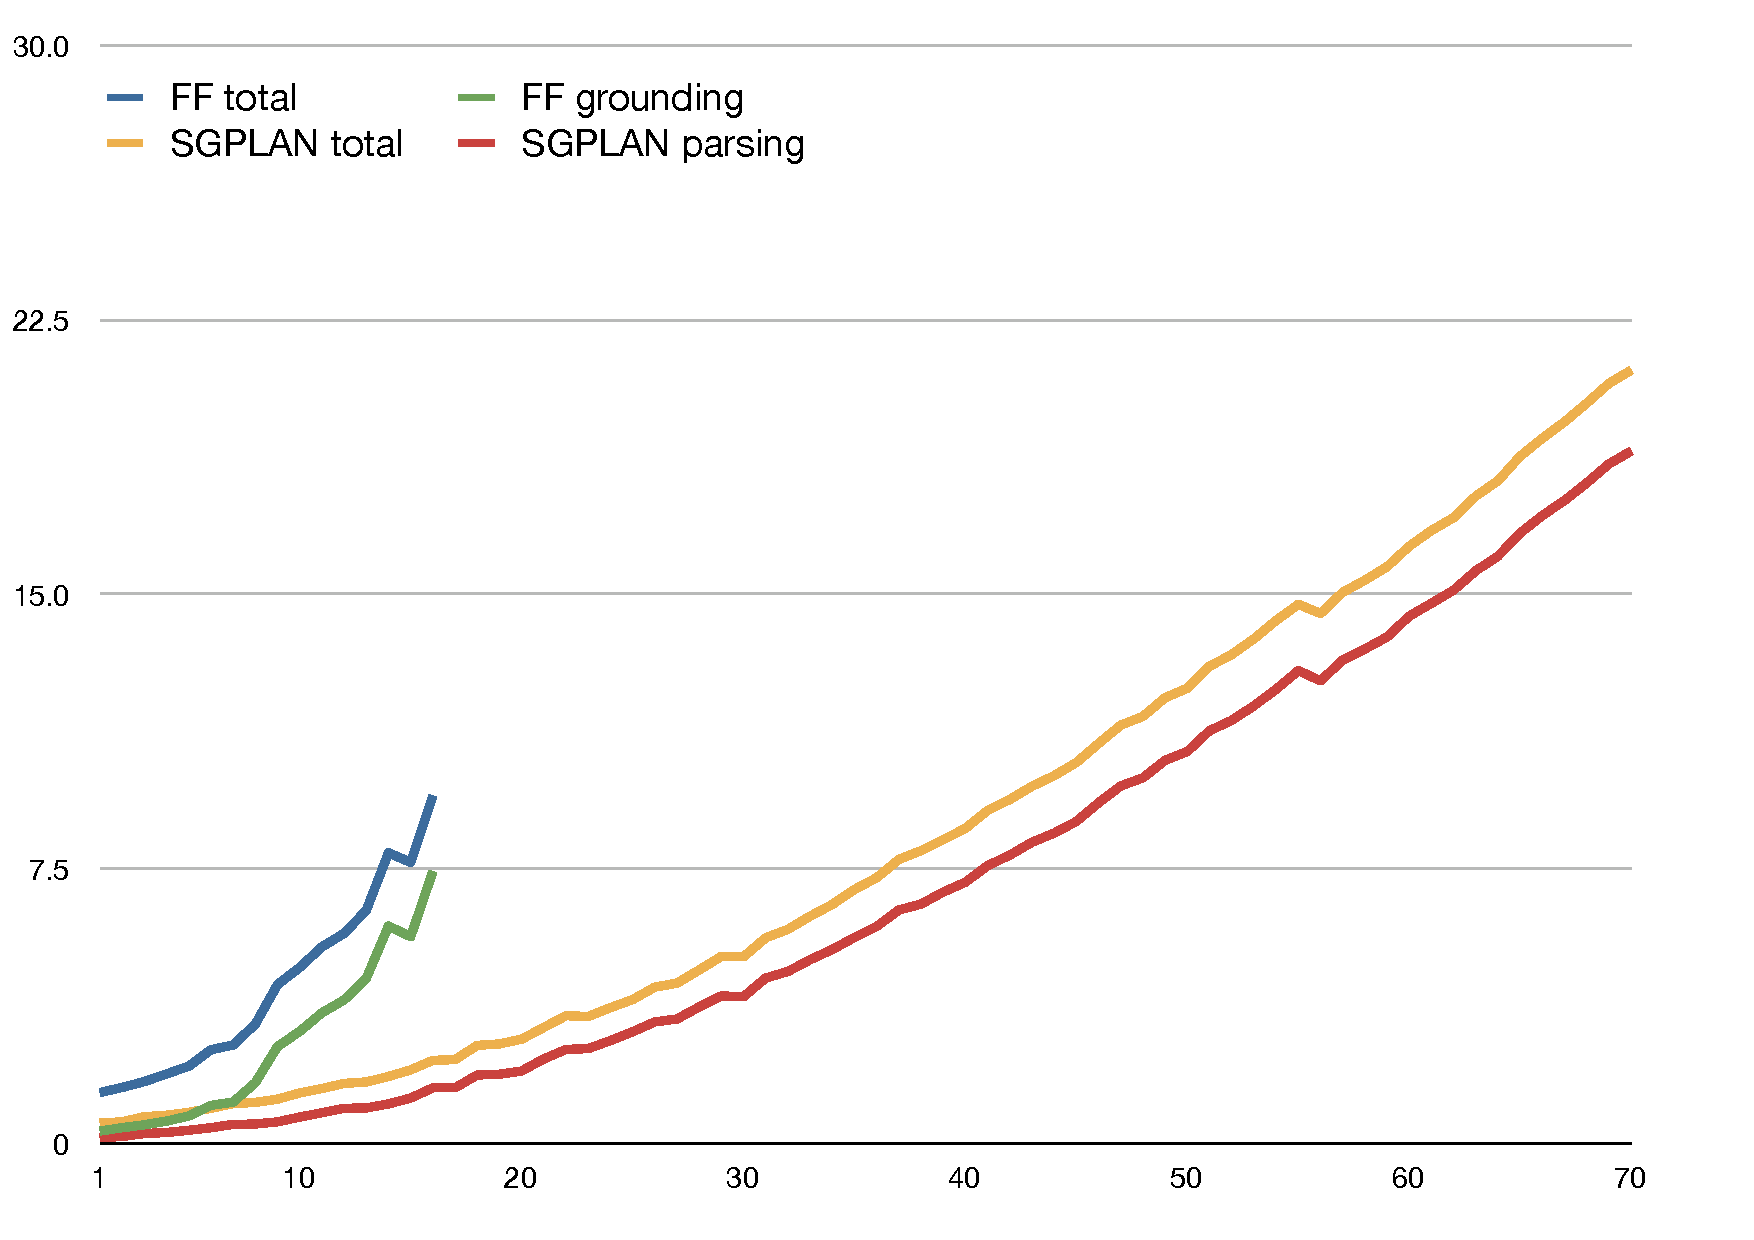
\includegraphics[width=1\columnwidth]{pic-runtime-empty-world}
  \caption{Results on the GIVE domain with junk
    positions for $h=20$ and $n=5$. The horizontal axis is $w$.
    The vertical axis is the runtime in seconds.}
  \label{fig:give-runtime-junk}
\end{figure}


\subsection{Experiment 4: GIVE worlds with inaccessible positions}
\label{sec:experiment-4:-give}

In the final experiment, we consider a variation on the GIVE worlds from
Experiment~3. As before, we begin with a base grid of $2n$ by $h$
positions, with buttons at positions $(2i-1,1)$ and $(2i,h)$ for $1 \leq i
\leq n$. We then generate a second grid of $w$ by $h$ positions and place
an additional button in this grid. Unlike Experiment~3, the second grid
does not extend the first grid but is ``disconnected'' so its positions are
inaccessible from the first grid, as shown in
Figure~\ref{fig:give-junk-nosoln}. Since the geometry of the grid makes it
impossible to construct a plan for pressing all the buttons in the world,
we instead investigate the time it takes a planner to arrive at the
conclusion that the problem cannot be solved.

Results for the $h=20$, $n=5$ case with $w$ ranging from 1 to 50 are shown
in Figure~\ref{fig:give-runtime-nosoln}.\footnote{FF and SGPLAN do
 not display runtimes when they fail to construct a plan so an external timing
 program was used to generate these results.}
In this case, the runtimes for FF rise sharply around $w=28$, producing
times that are unacceptable for an NLG system in practice. FF is unable
to complete problem instances above $w=35$. SGPLAN, by comparison, performs
exceptionally well and is able to complete problems instances up to $w=50$
in about 0.3 seconds and $w=80$ in about 0.6 seconds. These results
demonstrate that SGPLAN has a significant advantage over FF in this
experiment. 
%Our implementation of GraphPlan is unable to complete any of
%these problem instances.

\begin{figure}[t]
  \centering
  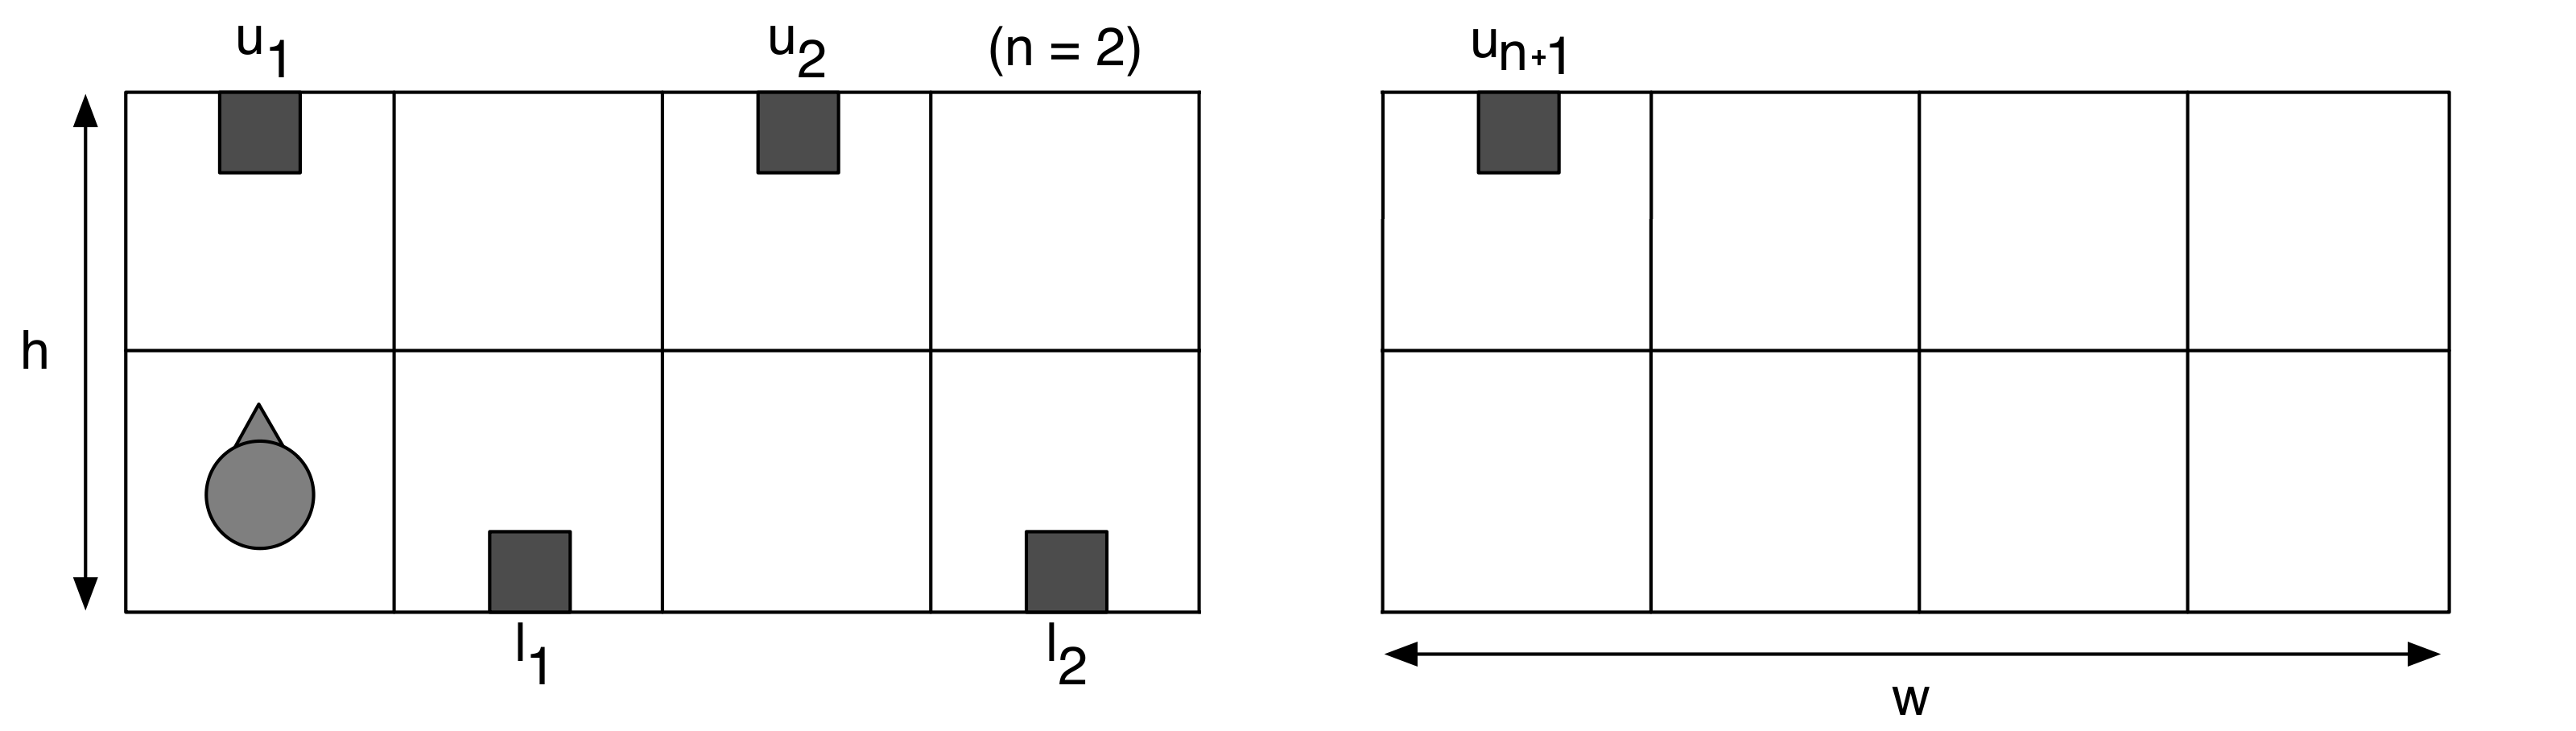
\includegraphics[width=0.85\columnwidth]{pic-empty-inaccessible}
  \caption{GIVE world with inaccessible positions.}
  \label{fig:give-junk-nosoln}
\end{figure}

\begin{figure}
  \centering
  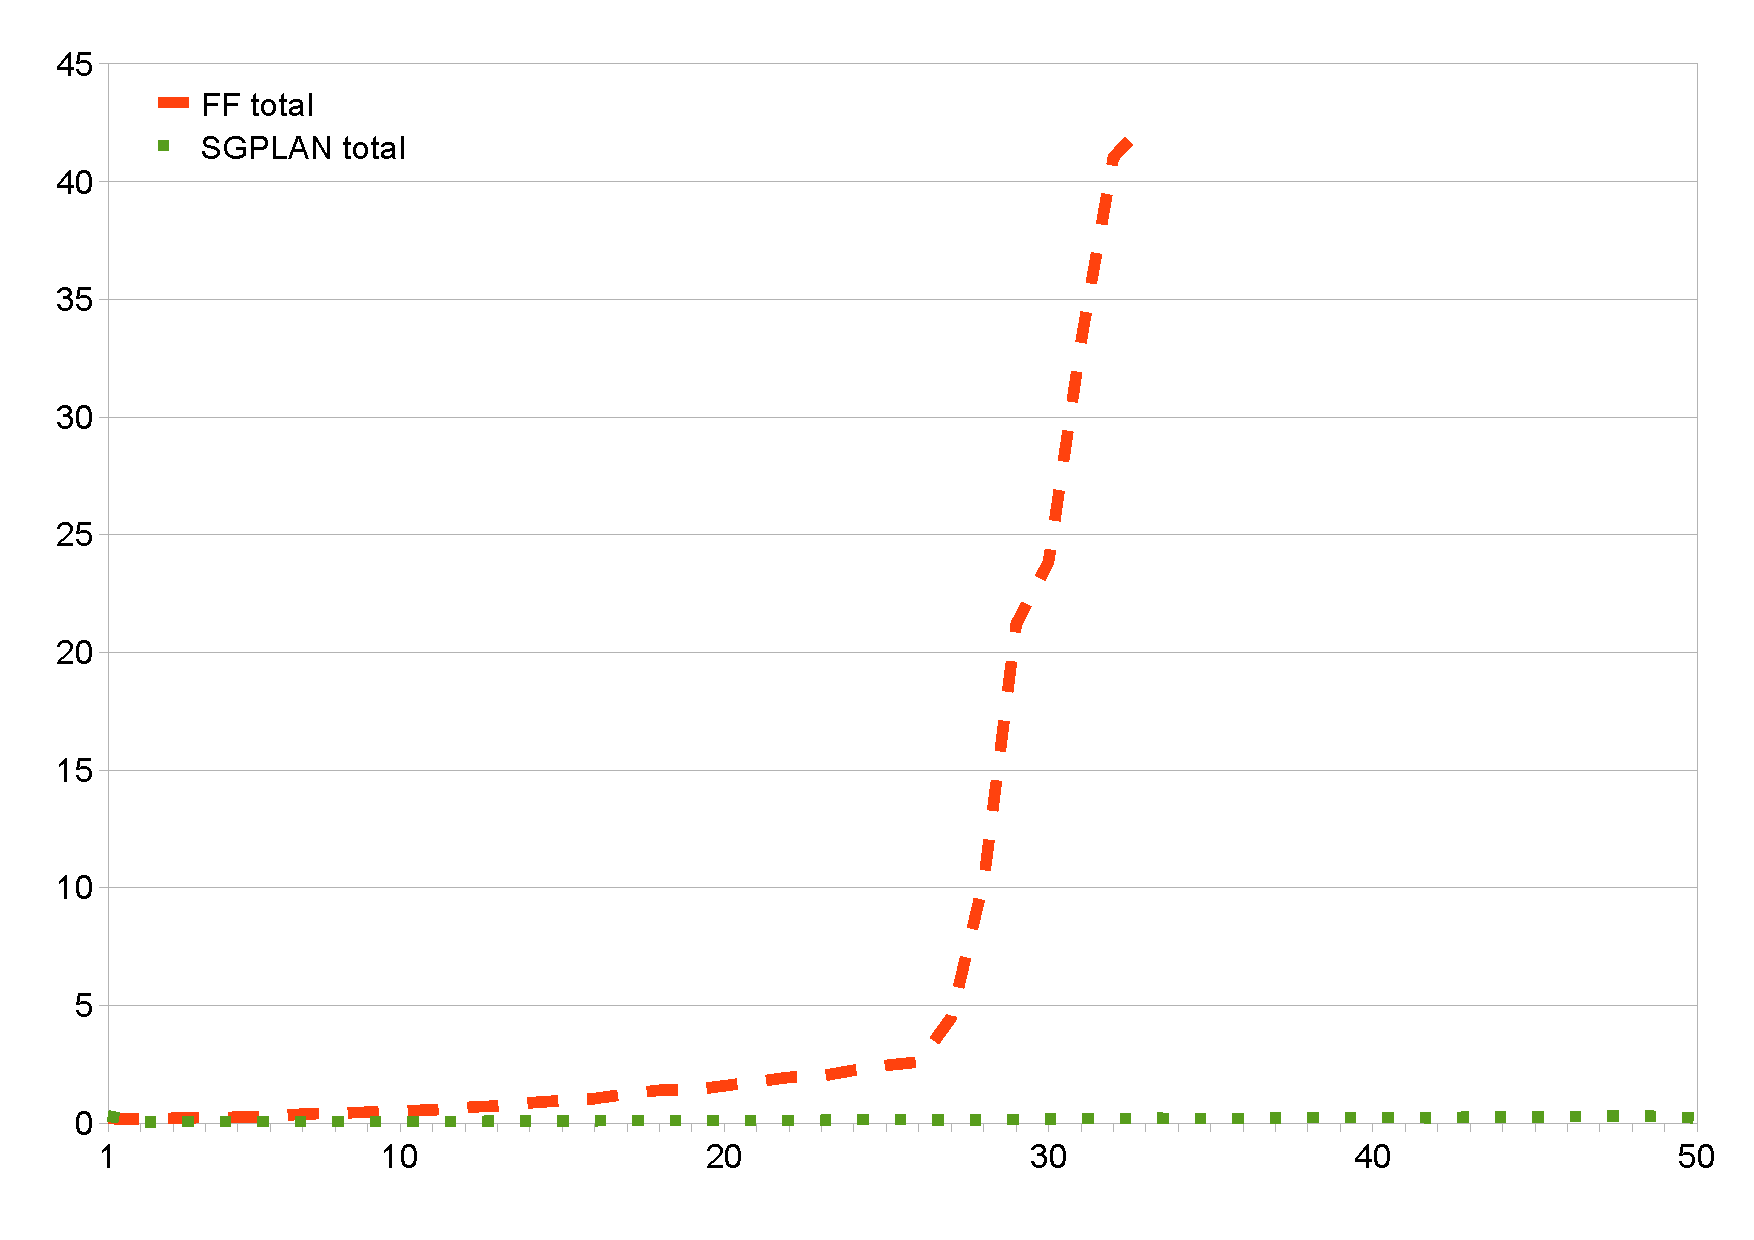
\includegraphics[width=0.85\columnwidth]{graph-exp4}
  %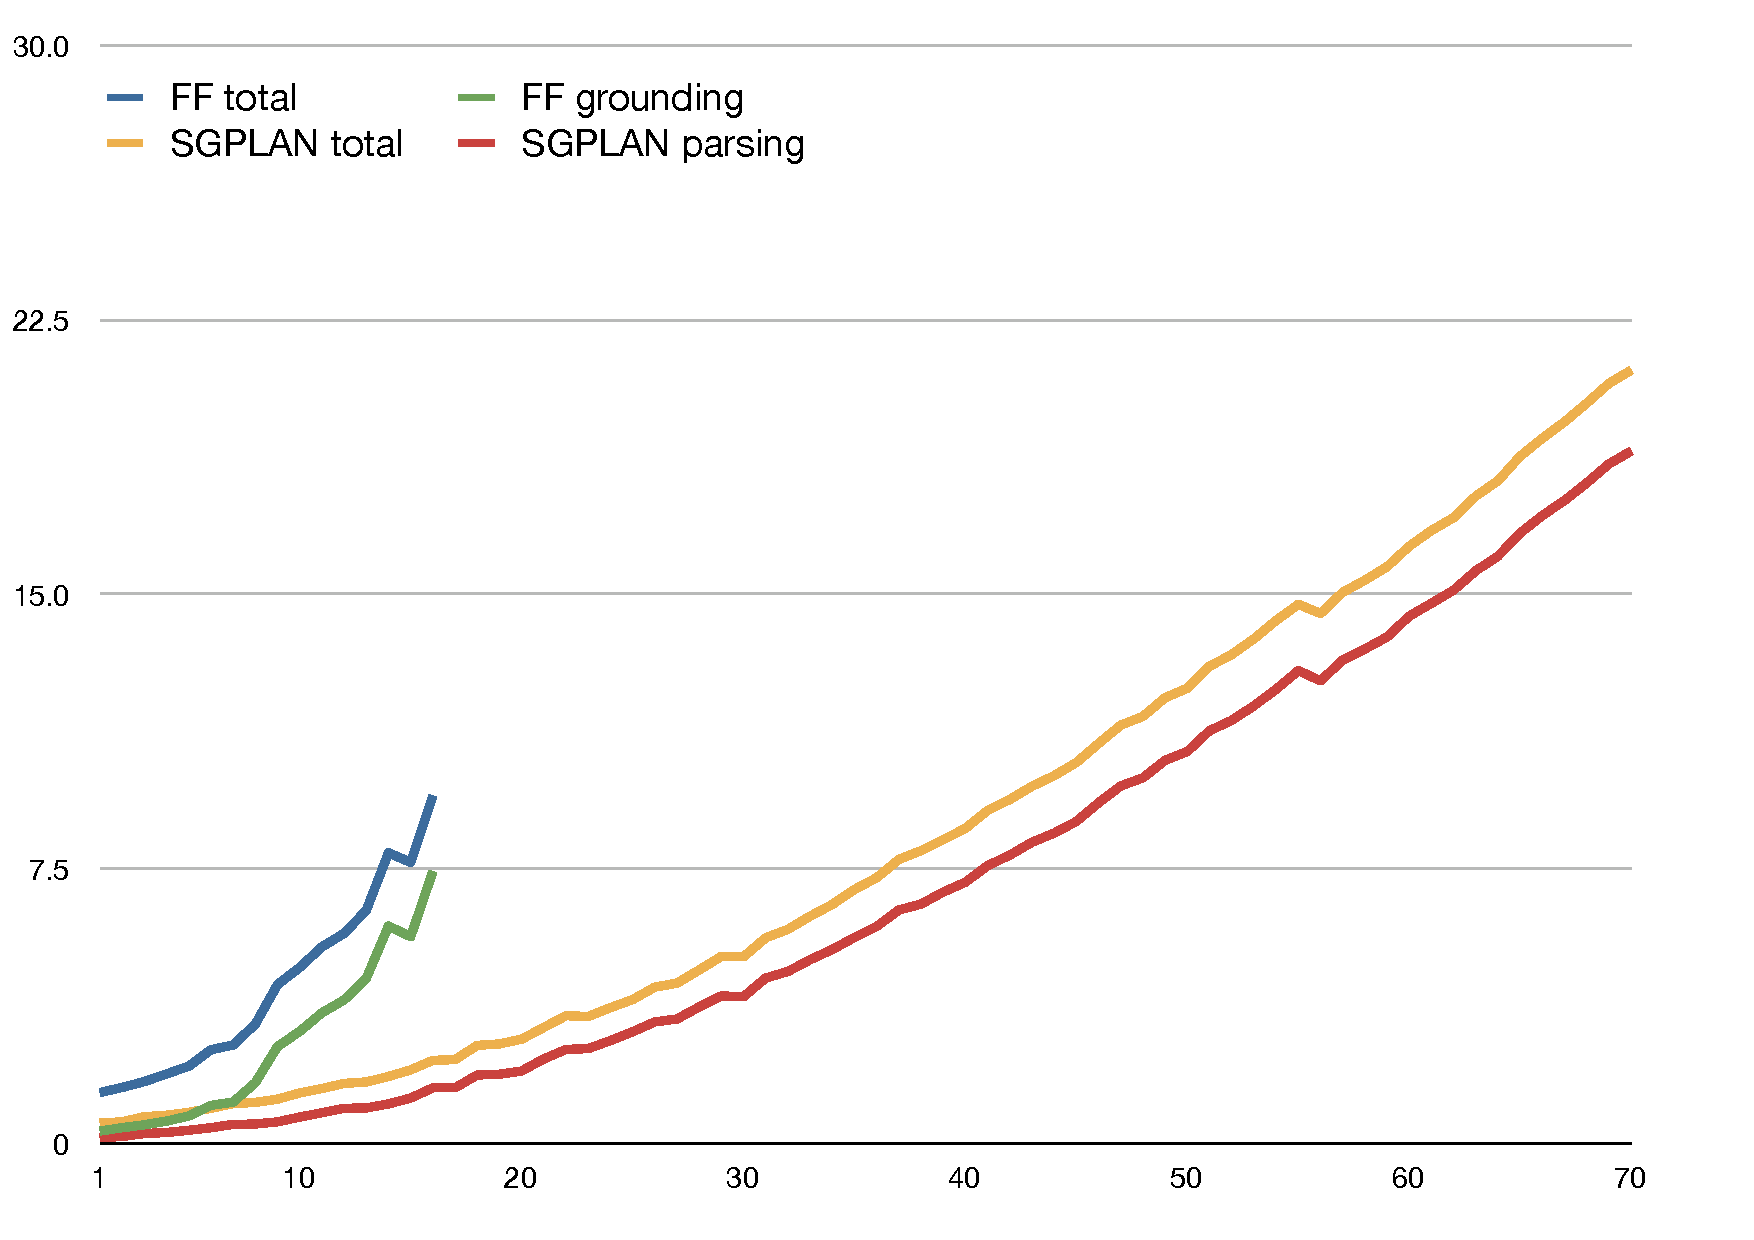
\includegraphics[width=1\columnwidth]{pic-runtime-empty-world}
  \caption{Results on the GIVE domain with inaccessible
    positions for $h=20$ and $n=5$. The horizontal axis is $w$.
    The vertical axis is the runtime in seconds.}
  \label{fig:give-runtime-nosoln}
\end{figure}

\section{Discussion}
\label{sec:discussion}

The positive conclusion we draw from our simple set of experiments is that
modern planners are fairly good at controlling the search for many of the
moderately-sized NLG problems we looked at. This is particularly true for
FF in the sentence generation domain, which generates nontrivial 14-word
sentences in about two seconds. Our results also indicate there is still
room for improvement, however: special-purpose algorithms are able to
generate much larger referring expressions in milliseconds
\citep{AreKolStr08}. Although search efficiency is not the main concern in
these domains, it nevertheless becomes a factor in scenarios like
Experiment~2, where the world is almost completely unconstrained and
(unsurprisingly) the search becomes much slower.

The most restrictive bottleneck in the two NLG domains we investigated is
the initial grounding step that many modern planners perform. While this
may be a good strategy for traditional planning benchmarks and IPC
domains---where plan length often dominates universe size and an initial
investment into grounding pays off in saved instantiations during
search---this approach has a very pronounced effect in domains like ours.
As our experiments show, there are natural planning domains in which
relatively short plans must be computed in large universes. For instance,
in the sentence generation domain, it is not unrealistic to look for plans
of length 20 over a universe consisting of thousands of domain individuals
and tens of thousands of possible action instantiations, some of which
require three domain individuals as parameters. Planners like FF and SGPLAN
are less effective in such domains, to the point that grounding
often dominates the total running time of these planners. (In the case of
Experiment~1, our ad-hoc implementation of GraphPlan outperforms both
planners in the sentence generation task.)

Since our domains are not that unusual in their structure and composition,
we hope that the lessons learned from our experiences can help improve the
performance of current planning systems. For instance, the common strategy
of splitting the universe into several types of individuals will not be a
very effective solution in our NLG domains given the large number of
individuals that could exist for a given type. On the other hand,
sophisticated techniques based on reachability analysis may have the
potential to improve this situation, provided such approaches can avoid the
drawbacks of unnecessary grounding.\footnote{See
  \citep{Bryce:07} for a good survey on reachability heuristics for planning
  graph-based approaches to plan generation.}
While recent trends in planning research have (rightfully) focused on the
development of algorithms that control search in sophisticated ways,
resulting in state-of-the-art planners that are more powerful and
successful than their predecessors, we nevertheless believe that
improvements are necessary if planning is to become a more mature
technology that can offer tools to a wider community of users and
researchers. At the end of the day, real-world users will care about the
\emph{total} runtime of a planner, which is more than just the search time.

By and large, our experiences with the planning community from a user's
point of view have been favourable. Thanks to the planning competitions, it
is easy to identify and download a fast state-of-the-art planner, at least
for Linux. However, in the course of our experiments we found and reported
bugs in both FF and SGPLAN. We also discovered that deciding as to which
planner is appropriate for a particular task is not always straightforward,
as the best performing planner in the IPC is not necessarily suitable for
every planning task. As our experiments have shown, even planners as
closely related as FF and SGPLAN can differ significantly in their
performance on different domains (for instance, our results in
Experiment~4).


\section{Conclusion}
\label{sec:conclusion}

In this paper, we introduced two novel planning domains arising from
problems in natural language generation: the sentence generation domain and
the Generating Instructions in Virtual Environments (GIVE) challenge
domain. We also reported the results of a set of experiments designed to
evaluate the suitability of off-the-shelf planners (particularly FF and
SGPLAN) in these domains.

Our results were mixed. While the planners we tested do an impressive job
of controlling the complexity of search in many domains, they also suffer
from practical problems that limit their performance in unexpected ways: in
both of our NLG domains the grounding step performed by FF and SGPLAN
dominates the time it takes to perform the search itself. As future work,
we hope to extend our analysis to other planners that do not perform the
initial grounding step, planners such as SHOP2
\citep{DBLP:journals/jair/NauAIKMWY03} that have traditionally performed
well on a wide range of domains, and new planners introduced in the latest
edition of the IPC.\footnote{See
 \url{http://ipc.informatik.uni-freiburg.de/} for details of the 2008
 International Planning Competition (deterministic track).}

The NLG community's recent interest in planning presents a valuable
opportunity for planning researchers. Domains like GIVE highlight certain
challenges, such as plan execution monitoring and plan presentation (i.e.,
summarisation and elaboration), but also offer a platform on which such
technologies can be evaluated in experiments with human users. Although we
have focused on classical planning problems in this work, research related
to reasoning under uncertainty, resource management, and planning with
knowledge and sensing, can also be investigated in these settings. As such,
we believe our domains would provide suitable challenges for planners
entered in future editions of the IPC. Provided some of the challenges we
have identified can be addressed, NLG-inspired problem domains offer a
constructive platform for the planning community to showcase their
techniques to a wider audience---and to improve the quality of their tools
for real-world planning tasks. 

\todo{planning claims general applicability; it's clear that IPC
  benchmarks focus areas of improvement; but it's not so clear to what
  extent this limits usefulness for non-IPC application areas; this
  paper evaluates this (for the first time??)}



\section*{Acknowledgements}

This work arose in the context of the Planning and Language Interest Group
at the University of Edinburgh. The authors would like to thank all members
of this group, especially Hector Geffner and Mark Steedman, for interesting
discussions. This work was partially supported by the DFG Research
Fellowship ``CRISP: Efficient integrated realization and microplanning''
and by the European Commission through the PACO-PLUS project
(FP6-2004-IST-4-27657).


\bibliography{references}
\bibliographystyle{ci}

\pagebreak
\listoffigures

\end{document}

